% Options for packages loaded elsewhere
% Options for packages loaded elsewhere
\PassOptionsToPackage{unicode}{hyperref}
\PassOptionsToPackage{hyphens}{url}
\PassOptionsToPackage{dvipsnames,svgnames,x11names}{xcolor}
%
\documentclass[
  12pt,
]{interact}
\usepackage{xcolor}
\usepackage{amsmath,amssymb}
\setcounter{secnumdepth}{5}
\usepackage{iftex}
\ifPDFTeX
  \usepackage[T1]{fontenc}
  \usepackage[utf8]{inputenc}
  \usepackage{textcomp} % provide euro and other symbols
\else % if luatex or xetex
  \usepackage{unicode-math} % this also loads fontspec
  \defaultfontfeatures{Scale=MatchLowercase}
  \defaultfontfeatures[\rmfamily]{Ligatures=TeX,Scale=1}
\fi
\usepackage{lmodern}
\ifPDFTeX\else
  % xetex/luatex font selection
\fi
% Use upquote if available, for straight quotes in verbatim environments
\IfFileExists{upquote.sty}{\usepackage{upquote}}{}
\IfFileExists{microtype.sty}{% use microtype if available
  \usepackage[]{microtype}
  \UseMicrotypeSet[protrusion]{basicmath} % disable protrusion for tt fonts
}{}
\usepackage{setspace}
\makeatletter
\@ifundefined{KOMAClassName}{% if non-KOMA class
  \IfFileExists{parskip.sty}{%
    \usepackage{parskip}
  }{% else
    \setlength{\parindent}{0pt}
    \setlength{\parskip}{6pt plus 2pt minus 1pt}}
}{% if KOMA class
  \KOMAoptions{parskip=half}}
\makeatother
% Make \paragraph and \subparagraph free-standing
\makeatletter
\ifx\paragraph\undefined\else
  \let\oldparagraph\paragraph
  \renewcommand{\paragraph}{
    \@ifstar
      \xxxParagraphStar
      \xxxParagraphNoStar
  }
  \newcommand{\xxxParagraphStar}[1]{\oldparagraph*{#1}\mbox{}}
  \newcommand{\xxxParagraphNoStar}[1]{\oldparagraph{#1}\mbox{}}
\fi
\ifx\subparagraph\undefined\else
  \let\oldsubparagraph\subparagraph
  \renewcommand{\subparagraph}{
    \@ifstar
      \xxxSubParagraphStar
      \xxxSubParagraphNoStar
  }
  \newcommand{\xxxSubParagraphStar}[1]{\oldsubparagraph*{#1}\mbox{}}
  \newcommand{\xxxSubParagraphNoStar}[1]{\oldsubparagraph{#1}\mbox{}}
\fi
\makeatother

\usepackage{color}
\usepackage{fancyvrb}
\newcommand{\VerbBar}{|}
\newcommand{\VERB}{\Verb[commandchars=\\\{\}]}
\DefineVerbatimEnvironment{Highlighting}{Verbatim}{commandchars=\\\{\}}
% Add ',fontsize=\small' for more characters per line
\usepackage{framed}
\definecolor{shadecolor}{RGB}{241,243,245}
\newenvironment{Shaded}{\begin{snugshade}}{\end{snugshade}}
\newcommand{\AlertTok}[1]{\textcolor[rgb]{0.68,0.00,0.00}{#1}}
\newcommand{\AnnotationTok}[1]{\textcolor[rgb]{0.37,0.37,0.37}{#1}}
\newcommand{\AttributeTok}[1]{\textcolor[rgb]{0.40,0.45,0.13}{#1}}
\newcommand{\BaseNTok}[1]{\textcolor[rgb]{0.68,0.00,0.00}{#1}}
\newcommand{\BuiltInTok}[1]{\textcolor[rgb]{0.00,0.23,0.31}{#1}}
\newcommand{\CharTok}[1]{\textcolor[rgb]{0.13,0.47,0.30}{#1}}
\newcommand{\CommentTok}[1]{\textcolor[rgb]{0.37,0.37,0.37}{#1}}
\newcommand{\CommentVarTok}[1]{\textcolor[rgb]{0.37,0.37,0.37}{\textit{#1}}}
\newcommand{\ConstantTok}[1]{\textcolor[rgb]{0.56,0.35,0.01}{#1}}
\newcommand{\ControlFlowTok}[1]{\textcolor[rgb]{0.00,0.23,0.31}{\textbf{#1}}}
\newcommand{\DataTypeTok}[1]{\textcolor[rgb]{0.68,0.00,0.00}{#1}}
\newcommand{\DecValTok}[1]{\textcolor[rgb]{0.68,0.00,0.00}{#1}}
\newcommand{\DocumentationTok}[1]{\textcolor[rgb]{0.37,0.37,0.37}{\textit{#1}}}
\newcommand{\ErrorTok}[1]{\textcolor[rgb]{0.68,0.00,0.00}{#1}}
\newcommand{\ExtensionTok}[1]{\textcolor[rgb]{0.00,0.23,0.31}{#1}}
\newcommand{\FloatTok}[1]{\textcolor[rgb]{0.68,0.00,0.00}{#1}}
\newcommand{\FunctionTok}[1]{\textcolor[rgb]{0.28,0.35,0.67}{#1}}
\newcommand{\ImportTok}[1]{\textcolor[rgb]{0.00,0.46,0.62}{#1}}
\newcommand{\InformationTok}[1]{\textcolor[rgb]{0.37,0.37,0.37}{#1}}
\newcommand{\KeywordTok}[1]{\textcolor[rgb]{0.00,0.23,0.31}{\textbf{#1}}}
\newcommand{\NormalTok}[1]{\textcolor[rgb]{0.00,0.23,0.31}{#1}}
\newcommand{\OperatorTok}[1]{\textcolor[rgb]{0.37,0.37,0.37}{#1}}
\newcommand{\OtherTok}[1]{\textcolor[rgb]{0.00,0.23,0.31}{#1}}
\newcommand{\PreprocessorTok}[1]{\textcolor[rgb]{0.68,0.00,0.00}{#1}}
\newcommand{\RegionMarkerTok}[1]{\textcolor[rgb]{0.00,0.23,0.31}{#1}}
\newcommand{\SpecialCharTok}[1]{\textcolor[rgb]{0.37,0.37,0.37}{#1}}
\newcommand{\SpecialStringTok}[1]{\textcolor[rgb]{0.13,0.47,0.30}{#1}}
\newcommand{\StringTok}[1]{\textcolor[rgb]{0.13,0.47,0.30}{#1}}
\newcommand{\VariableTok}[1]{\textcolor[rgb]{0.07,0.07,0.07}{#1}}
\newcommand{\VerbatimStringTok}[1]{\textcolor[rgb]{0.13,0.47,0.30}{#1}}
\newcommand{\WarningTok}[1]{\textcolor[rgb]{0.37,0.37,0.37}{\textit{#1}}}

\usepackage{longtable,booktabs,array}
\usepackage{calc} % for calculating minipage widths
% Correct order of tables after \paragraph or \subparagraph
\usepackage{etoolbox}
\makeatletter
\patchcmd\longtable{\par}{\if@noskipsec\mbox{}\fi\par}{}{}
\makeatother
% Allow footnotes in longtable head/foot
\IfFileExists{footnotehyper.sty}{\usepackage{footnotehyper}}{\usepackage{footnote}}
\makesavenoteenv{longtable}
\usepackage{graphicx}
\makeatletter
\newsavebox\pandoc@box
\newcommand*\pandocbounded[1]{% scales image to fit in text height/width
  \sbox\pandoc@box{#1}%
  \Gscale@div\@tempa{\textheight}{\dimexpr\ht\pandoc@box+\dp\pandoc@box\relax}%
  \Gscale@div\@tempb{\linewidth}{\wd\pandoc@box}%
  \ifdim\@tempb\p@<\@tempa\p@\let\@tempa\@tempb\fi% select the smaller of both
  \ifdim\@tempa\p@<\p@\scalebox{\@tempa}{\usebox\pandoc@box}%
  \else\usebox{\pandoc@box}%
  \fi%
}
% Set default figure placement to htbp
\def\fps@figure{htbp}
\makeatother


% definitions for citeproc citations
\NewDocumentCommand\citeproctext{}{}
\NewDocumentCommand\citeproc{mm}{%
  \begingroup\def\citeproctext{#2}\cite{#1}\endgroup}
\makeatletter
 % allow citations to break across lines
 \let\@cite@ofmt\@firstofone
 % avoid brackets around text for \cite:
 \def\@biblabel#1{}
 \def\@cite#1#2{{#1\if@tempswa , #2\fi}}
\makeatother
\newlength{\cslhangindent}
\setlength{\cslhangindent}{1.5em}
\newlength{\csllabelwidth}
\setlength{\csllabelwidth}{3em}
\newenvironment{CSLReferences}[2] % #1 hanging-indent, #2 entry-spacing
 {\begin{list}{}{%
  \setlength{\itemindent}{0pt}
  \setlength{\leftmargin}{0pt}
  \setlength{\parsep}{0pt}
  % turn on hanging indent if param 1 is 1
  \ifodd #1
   \setlength{\leftmargin}{\cslhangindent}
   \setlength{\itemindent}{-1\cslhangindent}
  \fi
  % set entry spacing
  \setlength{\itemsep}{#2\baselineskip}}}
 {\end{list}}
\usepackage{calc}
\newcommand{\CSLBlock}[1]{\hfill\break\parbox[t]{\linewidth}{\strut\ignorespaces#1\strut}}
\newcommand{\CSLLeftMargin}[1]{\parbox[t]{\csllabelwidth}{\strut#1\strut}}
\newcommand{\CSLRightInline}[1]{\parbox[t]{\linewidth - \csllabelwidth}{\strut#1\strut}}
\newcommand{\CSLIndent}[1]{\hspace{\cslhangindent}#1}



\setlength{\emergencystretch}{3em} % prevent overfull lines

\providecommand{\tightlist}{%
  \setlength{\itemsep}{0pt}\setlength{\parskip}{0pt}}



 


\usepackage{amsmath}
\usepackage{amssymb}
\usepackage{fvextra}
\DefineVerbatimEnvironment{verbatim}{Verbatim}{breaklines=true, breakanywhere=true, breakindent=1em, fontsize=\small}
\DefineVerbatimEnvironment{Highlighting}{Verbatim}{commandchars=\\\{\}, breaklines=true, breakanywhere=true, breakindent=1em, fontsize=\small}
\makeatletter
\AtBeginDocument{%
  \captionsetup[codelisting]{skip=-0.8em}%
  \renewenvironment{codelisting}{%
    \def\@captype{codelisting}%
    \par\addvspace{0.5em}\noindent
  }{%
    \par\addvspace{0.5em}%
  }%
}
\makeatother
\AtBeginDocument{\floatplacement{codelisting}{H}}
\usepackage{orcidlink}
\makeatletter
\@ifpackageloaded{caption}{}{\usepackage{caption}}
\AtBeginDocument{%
\ifdefined\contentsname
  \renewcommand*\contentsname{Table of contents}
\else
  \newcommand\contentsname{Table of contents}
\fi
\ifdefined\listfigurename
  \renewcommand*\listfigurename{List of Figures}
\else
  \newcommand\listfigurename{List of Figures}
\fi
\ifdefined\listtablename
  \renewcommand*\listtablename{List of Tables}
\else
  \newcommand\listtablename{List of Tables}
\fi
\ifdefined\figurename
  \renewcommand*\figurename{Figure}
\else
  \newcommand\figurename{Figure}
\fi
\ifdefined\tablename
  \renewcommand*\tablename{Table}
\else
  \newcommand\tablename{Table}
\fi
}
\@ifpackageloaded{float}{}{\usepackage{float}}
\floatstyle{ruled}
\@ifundefined{c@chapter}{\newfloat{codelisting}{h}{lop}}{\newfloat{codelisting}{h}{lop}[chapter]}
\floatname{codelisting}{Listing}
\newcommand*\listoflistings{\listof{codelisting}{List of Listings}}
\makeatother
\makeatletter
\makeatother
\makeatletter
\@ifpackageloaded{caption}{}{\usepackage{caption}}
\@ifpackageloaded{subcaption}{}{\usepackage{subcaption}}
\makeatother
\usepackage{bookmark}
\IfFileExists{xurl.sty}{\usepackage{xurl}}{} % add URL line breaks if available
\urlstyle{same}
\hypersetup{
  pdftitle={Code availability is not enough: schemas for documenting and extending data analysis},
  pdfauthor={H. Sherry Zhang; Roger D. Peng},
  pdfkeywords={Reproducibility, Large Language Models (LLMs), Data
analysis decisions, Many-analysts study, Statistical workflow},
  colorlinks=true,
  linkcolor={blue},
  filecolor={Maroon},
  citecolor={Blue},
  urlcolor={Blue},
  pdfcreator={LaTeX via pandoc}}


\title{Code availability is not enough: schemas for documenting and
extending data analysis}
\author{H. Sherry Zhang$\textsuperscript{1}$, Roger D.
Peng$\textsuperscript{1}$}

\thanks{CONTACT: H. Sherry
Zhang. Email: \href{mailto:hsherryzhang@utexas.edu}{\nolinkurl{hsherryzhang@utexas.edu}}. }
\begin{document}
\captionsetup{labelsep=space}
\maketitle
\textsuperscript{1} Department of Statistics and Data
Science, University of Texas at Austin, Texas, United States
\begin{abstract}
A data analysis involves a sequence of decisions, from data cleaning to
model specification, each of which can affect the reported result.
Reproducing that result is not the same as understanding the sequence of
decisions that produced it and the reasons for each: the code mixes
those decisions with implementation details, while the manuscript states
the major decisions and their rationale but scatters them across its
sections and often leaves out the minor ones. A reader may then ask how
the result would change under a different decision: the question itself
is easy to pose, but implementing it is often non-trivial in practice.
In this work, we propose a schema that represents a data analysis as a
collection of decisions in natural language, from which large language
models (LLMs) can generate and validate analysis scripts directly. This
workflow can also expand a single analysis into a full multiverse of
alternatives, specified in an alternative file, ready for comparison. We
demonstrate the proposed workflow in two applications. In the first, we
construct a schema for a published regression analysis of heaped smoking
data and show that it reproduces the reported estimates, and that a
reviewer-suggested alternative can be specified through the alternative
file and turned into code automatically. In the second, where no schema
is provided, we show how the workflow serves instead as a
reproducibility check, applied to the many-analysts football study. As
an intermediate representation between the manuscript and code scripts,
our schema gives a self-contained account of an analysis and makes it
extensible from a reader's perspective.
\end{abstract}
\begin{keywords}
\def\sep{;\ }
Reproducibility\sep Large Language Models (LLMs)\sep Data analysis
decisions\sep Many-analysts study\sep 
Statistical workflow
\end{keywords}


\setstretch{1.15}
\newpage

\section{Introduction}\label{sec-intro}

A data analysis is the product of a chain of decisions, from how the
data are cleaned to how the model is specified. {[}This chain of
decisions lets a reader comprehend the analysis, compare it against
other analyses of similar questions, question how the result would
change under an alternative decision.{]} Code and data availability, now
standard reproducible practice (Peng, 2011; Wrobel et al., 2024),
guarantee that the reported result can be reproduced, {[}but not the
chain of decisions that produced it.{]}

{[}Part of the reason is that{]} code and the decisions it implements
operate at different levels: code specifies precisely what a computer
should do, while a decision has a contextual interpretation that the
code itself does not capture. Consider a line such as
\texttt{dplyr::filter(df,\ x\ \textgreater{}\ 0)}, which has a precise
meaning as code: keep rows where \texttt{x} is positive. Which decision
this line encodes is not something the code can answer: it could
represent restricting the analysis to a subpopulation for which \$x
\textgreater{} 0 \$is substantively meaningful, or excluding
observations flagged as invalid by anencoding convention where \(x
\le 0\) denotes missingness, and nothing in the \texttt{filter()} syntax
indicates which is intended. Nor does code generally carry the rationale
behind a decision, unless the author has left detailed comments. A
better place to state the decisions is in the manuscript, where
decisions are described along with their rationale. But this information
is scattered across the manuscript rather than collected in one place,
with preprocessing and modelling decisions appearing in different
sections of the manuscript. Authors may also simply leave out decisions
they consider minor, on the assumption that the code provides all the
detail a reader would need. Reconstructing the full sequence, therefore,
means searching across the paper and the code for decisions and their
rationale before a reader can begin to comprehend the analysis. Ideally,
this sequence of decisions and their rationale would live in a single
file, so a reader can follow the analysis directly rather than piecing
it together from multiple sources. This file should also be extensible,
so a reader can specify an alternative decision and easily evaluate it
to see how the result would change.

In this paper, we present a schema designed to describe data analysis
{[}in a structured way that captures the decisions and their rationale,
as well as the inputs and outputs of each step{]}. We also demonstrate
how this schema, coupled with LLMs, can be used to generate code scripts
from natural-language descriptions in manuscripts, and explore
alternative decision choices. We present two applications. The first
takes the perspective of an author supplying a schema alongside a
published manuscript, using the GAITD regression analysis of heaped
smoking data in Yee et al. (2025). A reader can then specify an
alternative file, coupled with the original schema, to compare model
performance under a different inflation-alteration specification. The
second, the many-analysts football study, considers the opposite
situation, where no schema is supplied and the workflow serves instead
as a reproducibility test. It extracts a schema from a simplified
version of each team's report, generates and validates the corresponding
code, and compares the result against that team's published estimate.
This comparison also uncovers an inconsistency in one team's published
report between the covariate described in the text and the one implied
by their results. We further demonstrate how the schema supports
specification and exploration of three alternative random effect
structures for Team 5.

The paper is organized as follows: In Section~\ref{sec-method}, we
present our methodology, including the schema representation for
describing data analysis, the specification of the alternative file, and
the workflow for generating and validating code from the schema with
LLMs. In Section~\ref{sec-gaitd}, we construct a schema for a published
GAITD regression analysis and show how it allows a reader to evaluate an
alternative specification directly. In Section~\ref{sec-application}, we
apply the workflow as a reproducibility test to the many-analysts
football study, recovering the reported results for most teams and
discussing the failed cases. Finally, in Section~\ref{sec-discussion},
we discuss the implications of our work and potential future directions.

\section{Methodology}\label{sec-method}

As traditional reproducibility practices can be insufficient for
understanding complex modern data analyses, we have designed two
complementary YAML formats and the associated workflow to better support
comprehension and extensibility in applied data analysis. Our workflow
is designed to be 1) decision-centric: analyses are represented as a
sequence of decisions with explicit rationale, and 2) reader-oriented
exploration: readers can inspect, compare, and extend those decisions.

\subsection{A schema for describing data analysis}\label{sec-schema}

We represent a data analysis,
\(\mathcal{S} = \{A_1, A_2, \cdots, A_n\}\), as a sequence of \(n\)
analytical steps \(A_i\), applied to a dataset \(\mathcal{D}\), where
each step, \(A_i\), is defined as a tuple:

\begin{equation}
A_{i} = \langle f_{i}, \pi_{i}, \rho_{i}, \mathcal{I}_{i}, \mathcal{O}_{i}, \omega_{i} \rangle.
\end{equation}

The components of \(A_i\) can be partitioned into two parts: a required
triplet \((f_{i}, \pi_{i}, \rho_{i})\) and an optional triplet
\((\mathcal{I}_{i}, \mathcal{O}_{i}, \omega_{i})\). The first component
of the triplet, \(f_{i} \in \mathcal{F}\), is the \emph{objective} of a
step, identifying the problem the step is trying to solve and thereby
fixing the space of alternative decisions that could equally address it
(formally introduced in Section~\ref{sec-alternative}). The second
component, \(\pi_{i} \in \Pi\), is the \emph{decision} made to achieve
\(f_i\): it is a narration, in natural language, of what a corresponding
line of code would do, situated in the context of this specific
analysis, rather than the code's syntax itself. The term \(\rho_{i}\) is
the \emph{rationale} provided for choosing the decision \(\pi_{i}\) over
the other alternatives that could have fulfilled the same objective; it
is recorded in the \texttt{rationale} field of the schema. Structuring
this information into a schema involves defining the three components
described above for each step. As an example, consider the description
for calculating the Human Development Index (HDI) (United Nations
Development Programme, 2025):

\begin{enumerate}
\def\labelenumi{\arabic{enumi})}
\tightlist
\item
  Scale all four variables (life expectancy, expected years of
  schooling, mean years of schooling, and GNI per capita) to the {[}0,
  1{]} range.
\item
  Combine the two education variables (expected years of schooling and
  mean years of schooling) into a single education variable.
\item
  Combine the three dimensions (health, education, and income) into a
  single index using a geometric mean.
\end{enumerate}

In Step 3, the objective is to combine the three dimensions. While a
simple arithmetic mean could be an alternative decision to fulfill this
goal, the geometric mean (the decision) is chosen because it penalizes
uneven development among the three dimensions (the rationale). The full
schema for constructing HDI is presented in Listing~\ref{lst-schema}.

\begin{codelisting}

\caption{\label{lst-schema}An example schema for calculating Human
Development Index (HDI)}

\centering{

\begin{Shaded}
\begin{Highlighting}[]
\FunctionTok{meta}\KeywordTok{:}
\AttributeTok{  }\FunctionTok{type}\KeywordTok{:}\AttributeTok{ schema}
\FunctionTok{nodes}\KeywordTok{:}
\KeywordTok{{-}}\AttributeTok{ }\FunctionTok{id}\KeywordTok{:}\AttributeTok{ step{-}scaling}
\AttributeTok{  }\FunctionTok{objective}\KeywordTok{:}\AttributeTok{ how to handle variables in different scales?}
\AttributeTok{  }\FunctionTok{decision}\KeywordTok{:}\AttributeTok{ apply min{-}max scaling to each variable}
\AttributeTok{  }\FunctionTok{rationale}\KeywordTok{:}\AttributeTok{ to convert the variables to the same scale for future}
\AttributeTok{    construction of a single index}
\KeywordTok{{-}}\AttributeTok{ }\FunctionTok{id}\KeywordTok{:}\AttributeTok{ step{-}education}
\AttributeTok{  }\FunctionTok{objective}\KeywordTok{:}\AttributeTok{ how to combine the two education{-}related variables?}
\AttributeTok{  }\FunctionTok{decision}\KeywordTok{:}\AttributeTok{ take the average}
\AttributeTok{  }\FunctionTok{rationale}\KeywordTok{:}\AttributeTok{ the arithmetic mean allows perfect substitutability}
\AttributeTok{    between the two variables}
\KeywordTok{{-}}\AttributeTok{ }\FunctionTok{id}\KeywordTok{:}\AttributeTok{ step{-}combine}
\AttributeTok{  }\FunctionTok{objective}\KeywordTok{:}\AttributeTok{ how to combine the three dimensions into a single index?}
\AttributeTok{  }\FunctionTok{decision}\KeywordTok{:}\AttributeTok{ use the geometric mean}
\AttributeTok{  }\FunctionTok{rationale}\KeywordTok{:}\AttributeTok{ the geometric mean penalizes uneven development }
\AttributeTok{    among the three core dimensions}
\end{Highlighting}
\end{Shaded}

}

\end{codelisting}%

The required triplet \((f_i, \pi_i, \rho_i)\) is already sufficient on
its own for a human reader to follow the analytical logic of a step,
without needing access to the underlying dataset. The optional triplet
\((\mathcal{I}_i, \mathcal{O}_i, \omega_i)\) adds a further layer on top
of this: \(\mathcal{I}_i\) and \(\mathcal{O}_i\) bind the step to
concrete variables in the dataset, resolving ahead of time the variable
mapping that an LLM would otherwise have to infer at the point of code
generation. Populating them requires a dataset to be available, which is
why they remain optional rather than required. Because the schema is
meant to specify an analysis before the corresponding code is generated,
the output of a step can name a variable that does not yet exist in the
dataset; this is inherent to using the schema as a specification rather
than a post-hoc description of existing code. The inputs for any given
step, by contrast, must be within the existing data scope, comprising
variables in the original dataset and all outputs from previous steps.
In practice, \(\mathcal{O}_i\) most often names a column added to the
evolving dataset via non-standard evaluation, as in
\texttt{tidyverse}-style pipelines; a small number of steps, such as
model fitting, instead produce a distinct object that is not itself a
column of \(\mathcal{D}\). Formally, we require:

\[\mathcal{I}_{i} \subseteq \left( \mathcal{D} \cup \bigcup_{j < i} \mathcal{O}_{j} \right), \quad \forall i \in \{2, \dots, n\}.\]

When the schema is extracted automatically by Large Language Models
(LLMs) from text, the inputs and outputs will be inferred by the LLMs,
if a dataset is provided. We also introduce a categorical confidence
score, \(\omega_{i}\) (low, medium, high), defined as the model's
confidence that the recorded \((f_i, \pi_i, \rho_i)\) correctly reflects
the source text; \(\omega_i\) is low precisely when one or more of these
components could not be read off the text directly and had to be
inferred by the LLM. Unlike the other components, \(\omega_i\) is not
part of the account of the analysis that a reader consumes; it is
consumed by the implementation, which uses it to flag steps for the
author to review or to prompt for clarification before the schema is
treated as settled.

Recording a step's decision \(\pi_i\) does not mean it is the only one
that could satisfy its objective \(f_i\): a reader may want to revisit
the decision made for some of these steps and consider alternatives that
address the same objective, a possibility we formalize next.

\subsection{Describing alternatives}\label{sec-alternative}

Another analyst following the HDI schema in Listing~\ref{lst-schema}
might wonder whether the reported index would look different under a
different decision at some step. Enumerating such choices is the premise
of multiverse analysis, and tooling exists to support it: the
\texttt{multiverse} package, for instance, lets an analyst declare
alternative branches inside an R notebook and expands them into the full
set of analyses (Sarma et al., 2023). What that tooling requires is code
--- each branch is expressed in the language the analysis is written in,
by someone able to write it. Our alternatives are specified at the level
of decisions instead, in natural language, and the code for each is
generated afterwards. The difference matters most for who can pose the
question: a multiverse is normally built by the original analyst while
exploring their own garden of forking paths, whereas an alternative file
can be written by a reader after publication, against a schema the
author has already supplied. Formally, a step in the schema can have a
candidate set of alternatives: step \(i\) may admit \(k_i\) decisions
that all satisfy its objective \(f_i\), \(\{A_i^1, \dots, A_i^{k_i}\}\),
of which the decision \(\pi_i\) recorded in the schema is just one
member, \(A_i^1\). An alternative file specifies the remaining
candidates, \(A_i^2, \dots, A_i^{k_i}\), for a subset of steps
\(C \subseteq \{1, \dots, n\}\).

The overall structure of an alternative file is shown in
Listing~\ref{lst-alternatives-skeleton}. The \texttt{meta} field at the
top identifies the file as an alternative specification
(\texttt{type:\ alternatives}), and the file-level \texttt{branch}
field, either \texttt{single} or \texttt{multi}, determines how the
candidates at each step combine, described below. The file itself is
organized as a list, one entry per step in \(C\) (\texttt{nodes} in the
YAML): each entry names its step in the original schema (via
\texttt{overrides}) and lists the alternative decisions for that step,
together with their rationale.

\begin{codelisting}

\caption{\label{lst-alternatives-skeleton}The skeleton of an alternative
YAML file, which consists of a \texttt{branch} mode and a list of
covered steps, each specifying a step in the original schema and its
alternative decisions.}

\centering{

\begin{Shaded}
\begin{Highlighting}[]
\FunctionTok{meta}\KeywordTok{:}
\AttributeTok{  }\FunctionTok{type}\KeywordTok{:}\AttributeTok{ alternatives}
\AttributeTok{  }\FunctionTok{branch}\KeywordTok{:}\AttributeTok{ single | multi}
\FunctionTok{nodes}\KeywordTok{:}
\AttributeTok{  }\KeywordTok{{-}}\AttributeTok{ }\FunctionTok{overrides}\KeywordTok{:}\AttributeTok{ \textless{}step id\textgreater{}}
\AttributeTok{    }\FunctionTok{alternatives}\KeywordTok{:}
\AttributeTok{      }\KeywordTok{{-}}\AttributeTok{ }\FunctionTok{id}\KeywordTok{:}\AttributeTok{ \textless{}alternative id\textgreater{}}
\FunctionTok{        decision}\KeywordTok{: }\AttributeTok{\textless{}...}\CharTok{\textgreater{}}
\FunctionTok{        rationale}\KeywordTok{: }\AttributeTok{\textless{}...}\CharTok{\textgreater{}}
\AttributeTok{      }\KeywordTok{{-}}\AttributeTok{ }\FunctionTok{id}\KeywordTok{:}\AttributeTok{ \textless{}alternative id\textgreater{}}
\AttributeTok{        ...}
\AttributeTok{  }\KeywordTok{{-}}\AttributeTok{ }\FunctionTok{overrides}\KeywordTok{:}\AttributeTok{ \textless{}step id\textgreater{}}
\AttributeTok{    }\FunctionTok{alternatives}\KeywordTok{:}
\AttributeTok{      ...}
\AttributeTok{  ...}
\end{Highlighting}
\end{Shaded}

}

\end{codelisting}%

Under \texttt{branch:\ single}, every step is restricted to a single
candidate decision. These alternatives and the unchanged steps in the
original schema together form one new analysis. This is useful when an
analyst wants to see what a different, internally consistent analysis
touching several steps at once would look like.
Listing~\ref{lst-alternatives-single} fills in the skeleton to construct
such an alternative version of the HDI computation, using a harmonic
mean to combine the two education variables in Step 2 and an arithmetic
mean to combine the three dimensions in Step 3.

\begin{codelisting}

\caption{\label{lst-alternatives-single}A sample alternative file that
changes the decisions for Step 2 and Step 3 in calculating Human
Development Index (HDI) to use a harmonic mean and an arithmetic mean,
respectively.}

\centering{

\begin{Shaded}
\begin{Highlighting}[]
\FunctionTok{meta}\KeywordTok{:}
\AttributeTok{  }\FunctionTok{type}\KeywordTok{:}\AttributeTok{ alternatives}
\AttributeTok{  }\FunctionTok{branch}\KeywordTok{:}\AttributeTok{ single}
\FunctionTok{nodes}\KeywordTok{:}
\AttributeTok{  }\KeywordTok{{-}}\AttributeTok{ }\FunctionTok{overrides}\KeywordTok{:}\AttributeTok{ step{-}education}
\AttributeTok{    }\FunctionTok{alternatives}\KeywordTok{:}
\AttributeTok{      }\KeywordTok{{-}}\AttributeTok{ }\FunctionTok{id}\KeywordTok{:}\AttributeTok{ harmonic{-}mean}
\AttributeTok{        }\FunctionTok{decision}\KeywordTok{:}\AttributeTok{ take the harmonic mean of the two education variables}
\AttributeTok{        }\FunctionTok{rationale}\KeywordTok{:}\AttributeTok{ penalizes disparity between the two schooling measures}
\AttributeTok{          rather than allowing one to compensate for the other}
\AttributeTok{  }\KeywordTok{{-}}\AttributeTok{ }\FunctionTok{overrides}\KeywordTok{:}\AttributeTok{ step{-}combine}
\AttributeTok{    }\FunctionTok{alternatives}\KeywordTok{:}
\AttributeTok{      }\KeywordTok{{-}}\AttributeTok{ }\FunctionTok{id}\KeywordTok{:}\AttributeTok{ arith{-}mean}
\AttributeTok{        }\FunctionTok{decision}\KeywordTok{:}\AttributeTok{ use an arithmetic mean}
\AttributeTok{        }\FunctionTok{rationale}\KeywordTok{:}\AttributeTok{ a simple average of the three dimensions}
\end{Highlighting}
\end{Shaded}

}

\end{codelisting}%

Sometimes a reader instead wants to test a range of alternatives for one
or more steps independently. Under \texttt{branch:\ multi}, the
candidates at each covered step, along with that step's original
decision, are crossed to produce every combination. In
Listing~\ref{lst-alternatives-multi}, one alternative is specified for
the education step (the harmonic mean) and two for the combination step
(an arithmetic mean and the minimum of the three dimensions). Together
with the original schema, this produces \((1+1) \times (2+1) = 6\)
analyses. More generally, with \(k_i\) candidates at each step
\(i \in C\), crossing all candidates yields \(\prod_{i \in C} k_i\)
analyses.

\begin{codelisting}

\caption{\label{lst-alternatives-multi}A sample alternative file that
explores one alternative decision for Step 2 and two for Step 3 in
calculating Human Development Index (HDI). Combining these alternatives
with the original schema produces a total of six (1+1) × (2+1) = 6
analyses.}

\centering{

\begin{Shaded}
\begin{Highlighting}[]
\FunctionTok{meta}\KeywordTok{:}
\AttributeTok{  }\FunctionTok{type}\KeywordTok{:}\AttributeTok{ alternatives}
\AttributeTok{  }\FunctionTok{branch}\KeywordTok{:}\AttributeTok{ multi}
\FunctionTok{nodes}\KeywordTok{:}
\AttributeTok{  }\KeywordTok{{-}}\AttributeTok{ }\FunctionTok{overrides}\KeywordTok{:}\AttributeTok{ step{-}education}
\AttributeTok{    }\FunctionTok{alternatives}\KeywordTok{:}
\AttributeTok{      }\KeywordTok{{-}}\AttributeTok{ }\FunctionTok{id}\KeywordTok{:}\AttributeTok{ harmonic{-}mean}
\AttributeTok{        }\FunctionTok{decision}\KeywordTok{:}\AttributeTok{ take the harmonic mean of the two education variables}
\AttributeTok{        }\FunctionTok{rationale}\KeywordTok{:}\AttributeTok{ penalizes disparity between the two schooling measures}
\AttributeTok{          rather than allowing one to compensate for the other}
\AttributeTok{  }\KeywordTok{{-}}\AttributeTok{ }\FunctionTok{overrides}\KeywordTok{:}\AttributeTok{ step{-}combine}
\AttributeTok{    }\FunctionTok{alternatives}\KeywordTok{:}
\AttributeTok{      }\KeywordTok{{-}}\AttributeTok{ }\FunctionTok{id}\KeywordTok{:}\AttributeTok{ arith{-}mean}
\AttributeTok{        }\FunctionTok{decision}\KeywordTok{:}\AttributeTok{ use an arithmetic mean}
\AttributeTok{        }\FunctionTok{rationale}\KeywordTok{:}\AttributeTok{ a simple average of the three dimensions}
\AttributeTok{      }\KeywordTok{{-}}\AttributeTok{ }\FunctionTok{id}\KeywordTok{:}\AttributeTok{ min{-}agg}
\AttributeTok{        }\FunctionTok{decision}\KeywordTok{:}\AttributeTok{ use the minimum of the three dimensions}
\AttributeTok{        }\FunctionTok{rationale}\KeywordTok{:}\AttributeTok{ a "weakest{-}link" aggregation that penalizes any single}
\AttributeTok{          lagging dimension more strongly than an average would}
\end{Highlighting}
\end{Shaded}

}

\end{codelisting}%

\subsection{Workflow}\label{workflow}

The overall workflow for schema-based data analysis is illustrated in
Figure~\ref{fig-workflow}. A schema can be created either manually from
the template or automatically by an LLM from a natural-language
manuscript. Once created, the schema serves as a structured
specification that guides a second LLM in generating the code for the
analysis. While the latest LLMs can generate reasonable code from a
prompt, they do not consistently achieve perfect accuracy. To improve
reliability, our design includes a third LLM agent responsible for code
validation. The validation process runs the generated script in a
sandbox environment and, if an error occurs, this agent is employed to
diagnose the script. The validation agent receives the generated code
together with the error message and the corresponding line number
produced during the execution, and returns a newer version of the
script. The revised script is then re-executed in the sandbox and this
cycle continues until one of the three conditions is met: the code runs
successfully, a maximum number of attempts is reached, or the user
terminates the process. Validation in this sense establishes that the
script executes to completion without error; it does not establish that
the code correctly implements the decisions recorded in the schema, and
a script can therefore pass validation while still departing from the
intended analysis. As shown in Section~\ref{sec-application}, this
process resolves the majority of R syntax issues encountered during data
wrangling and statistical modelling tasks, though we also encounter
cases where it does not. On top of supporting a single analytical
specification, the workflow also allows users to augment a schema with
an alternative YAML file. This expands the original schema into a
multiverse of parallel schemas, each representing a different sequence
of decision choices. The same code generation and validation workflow is
then applied independently to each schema, producing a corresponding set
of validated scripts.

\begin{figure}

\centering{

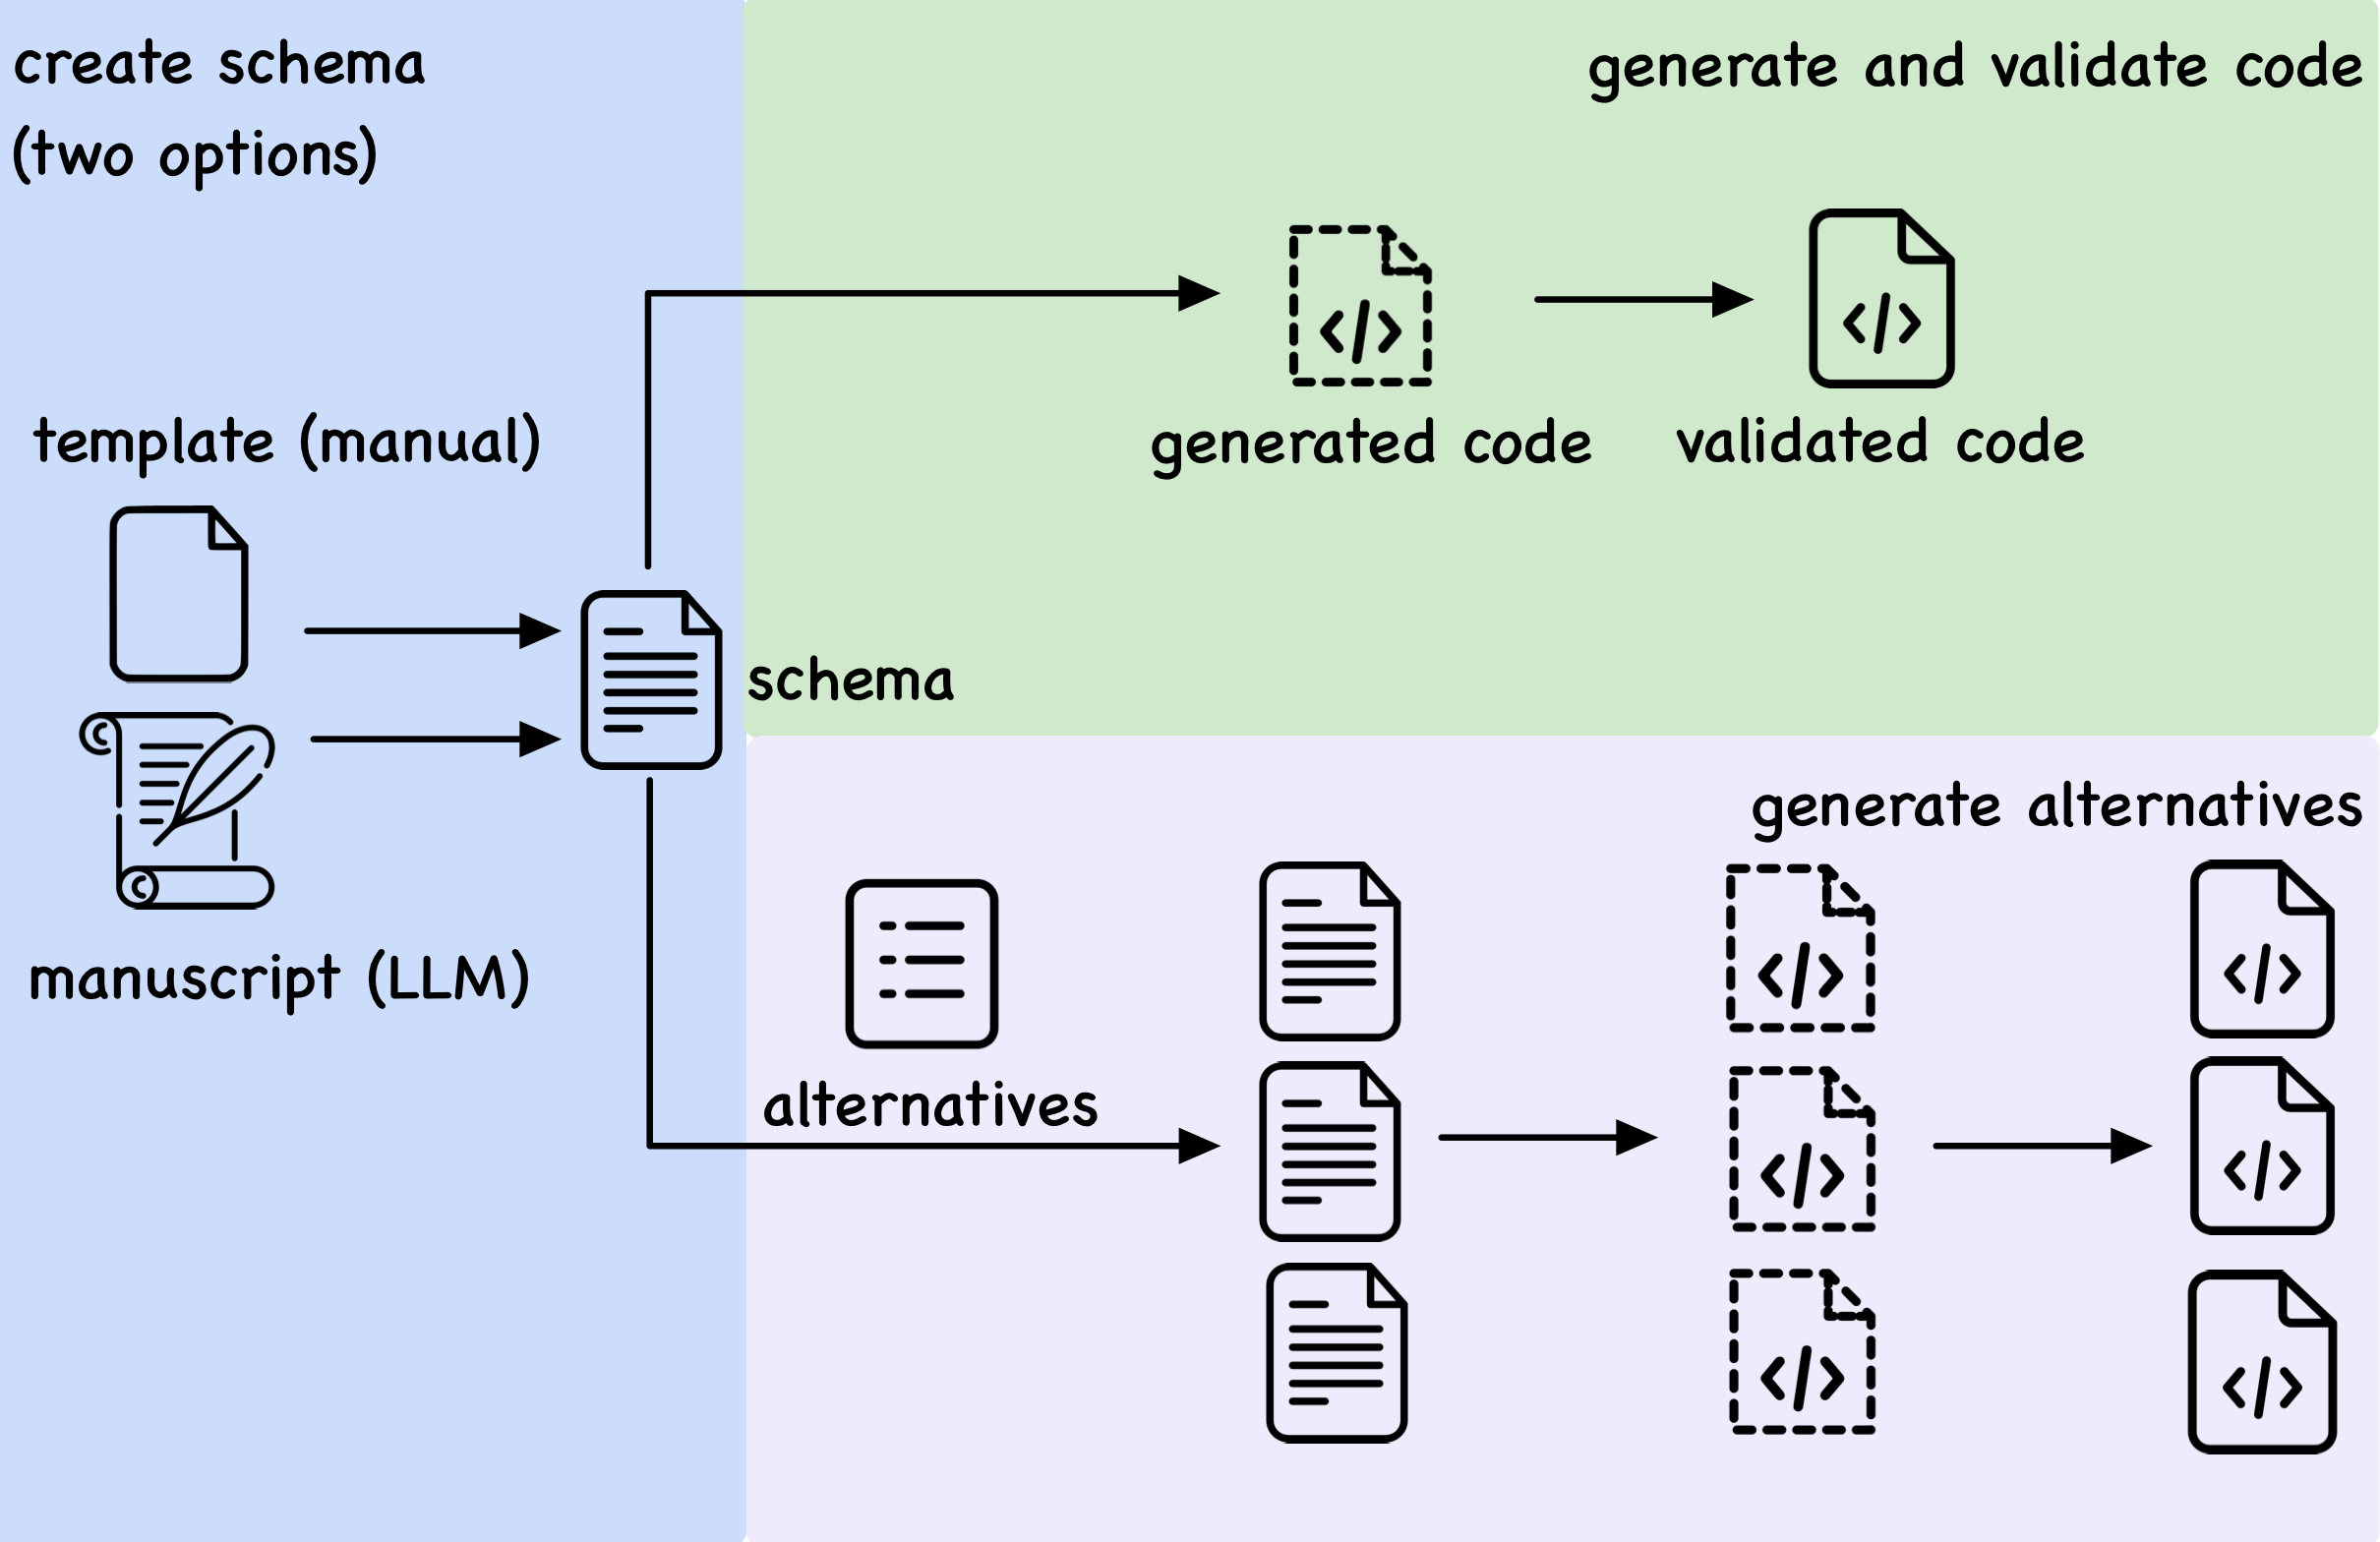
\includegraphics[width=1\linewidth,height=\textheight,keepaspectratio]{figures/workflow.png}

}

\caption{\label{fig-workflow}Overview of the schema-driven analysis
workflow. Schemas can be authored manually or generated from natural
language manuscripts by an LLM. Schemas are used to generate code, which
is validated through iterative execution in a sandboxed environment and
repaired when errors occur. Alternative specifications can expand a
schema into a multiverse of parallel analyses.}

\end{figure}%

Returning to the HDI example, the proposed workflow allows both authors
and readers to interact with a data analysis through natural language.
The schema in Listing~\ref{lst-schema} is straightforward to construct
from a template and can be included as supplementary material to
document the analytical workflow. An author may use the ``code
generation and validation'' path in Figure~\ref{fig-workflow} to
automatically generate the analysis script for computing HDI and
validate its accuracy. A reader, on the other hand, may wish to explore
how the HDI values or country rankings change if an arithmetic mean is
used instead of the original geometric mean. By combining the original
schema in Listing~\ref{lst-schema} with the alternative specification in
Listing~\ref{lst-alternatives-multi}, the ``alternative generation''
path produces a corresponding analysis script for each alternative with
LLMs. In contrast, modifying an existing code script by hand typically
requires manually coordinating changes across upstream and downstream
code. By representing analyses as a sequence of structured analytical
decisions, our workflow allows LLMs to automate much of this process,
making it easier to understand the sequence of steps taken in the
analysis and to explore alternatives.

\section{Application: GAITD regression of heaped smoking
data}\label{sec-gaitd}

In this section, we demonstrate the schema workflow from an author's
perspective: what it looks like for an author to provide a schema
alongside a manuscript, and what that then lets an audience do to
question and explore the analysis with much less effort than the
manuscript and its code alone would require. We use Yee et al. (2025)'s
GAITD regression analysis of heaped smoking data, published in the
Annals of Applied Statistics, as the example. Yee et al. (2025) report
four separate smoking-related responses; for demonstration purposes we
build the schema for only the first, smoking initiation age (P1, Section
5.1 of their paper), and the same workflow extends to the other three.

Listing~\ref{lst-heaping} contains fourteen entries; rather than list
them all, we highlight one as representative of what each entry records.
Every entry follows the \emph{objective}, \emph{decision}, and
\emph{rationale} structure introduced in Section~\ref{sec-schema}.
Consider \texttt{special\_value\_mid\_risk}: the decision is to treat
ages 12-14 and 19-21 as one inflated group with extra probability mass,
since these ages show a moderate, secondary elevation in the spikeplots,
surrounding the sharper peak already attributed to the high-risk group
(ages 15-18). Recording the rationale along with the decision allows a
reader to agree or disagree with the authors' choice, and to question
and explore the analysis, as we do later in this section. The other
thirteen entries follow the same structure.

\begin{codelisting}

\caption{\label{lst-heaping}A schema for the GAITD regression analysis
of smoking initiation age in Yee et al. (2025), constructed from the
manuscript and intended to be provided alongside it as a self-contained
account of the analysis.}

\centering{

\begin{Shaded}
\begin{Highlighting}[]
\FunctionTok{meta}\KeywordTok{:}
\AttributeTok{  }\FunctionTok{type}\KeywordTok{:}\AttributeTok{ schema}
\FunctionTok{nodes}\KeywordTok{:}
\KeywordTok{{-}}\AttributeTok{ }\FunctionTok{id}\KeywordTok{:}\AttributeTok{ complete\_case\_filtering}
\AttributeTok{  }\FunctionTok{objective}\KeywordTok{:}\AttributeTok{ handle missing data in selected variables}
\AttributeTok{  }\FunctionTok{decision}\KeywordTok{:}\AttributeTok{ apply complete{-}case filtering to all columns except TC30, TCquit, and SCA which have NAs by design}
\AttributeTok{  }\FunctionTok{rationale}\KeywordTok{:}\AttributeTok{ TC30, TCquit, and SCA are exempted from the completeness check since they are interlaced with NAs by design (e.g., SCA being NA means the person has not yet quit, a valid state rather than missingness); every other selected column is required to be non{-}missing because most smoking studies adjust for age, marital status, education and race, and this analysis follows suit. }

\KeywordTok{{-}}\AttributeTok{ }\FunctionTok{id}\KeywordTok{:}\AttributeTok{ age\_restriction}
\AttributeTok{  }\FunctionTok{objective}\KeywordTok{:}\AttributeTok{ define the age range for analysis}
\AttributeTok{  }\FunctionTok{decision}\KeywordTok{:}\AttributeTok{ restrict analysis to respondents aged less than 80 years (age \textless{} 80)}
\AttributeTok{  }\FunctionTok{rationale}\KeywordTok{:}\AttributeTok{ age was right{-}censored at 80}

\KeywordTok{{-}}\AttributeTok{ }\FunctionTok{id}\KeywordTok{:}\AttributeTok{ data\_quality\_correction}
\AttributeTok{  }\FunctionTok{objective}\KeywordTok{:}\AttributeTok{ handle logically impossible self{-}reported values}
\AttributeTok{  }\FunctionTok{decision}\KeywordTok{:}\AttributeTok{ set both SCA and SIA to NA where SCA {-} SIA \textless{} 0}
\AttributeTok{  }\FunctionTok{rationale}\KeywordTok{:}\AttributeTok{ quitting age before smoking initiation age is a logical impossibility and such values cannot be trusted}

\KeywordTok{{-}}\AttributeTok{ }\FunctionTok{id}\KeywordTok{:}\AttributeTok{ impute\_marital\_young}
\AttributeTok{  }\FunctionTok{objective}\KeywordTok{:}\AttributeTok{ assign a defensible marital status for young respondents, regardless of what was recorded}
\AttributeTok{  }\FunctionTok{decision}\KeywordTok{:}\AttributeTok{ recode marital status to "Never married" for everyone age \textless{} 20}
\AttributeTok{  }\FunctionTok{rationale}\KeywordTok{:}\AttributeTok{ this age group is effectively certain to have never been married, so the value is set by age rather than trusting the raw survey response}

\KeywordTok{{-}}\AttributeTok{ }\FunctionTok{id}\KeywordTok{:}\AttributeTok{ impute\_education\_young}
\AttributeTok{  }\FunctionTok{objective}\KeywordTok{:}\AttributeTok{ assign a defensible education category for young respondents, regardless of what was recorded}
\AttributeTok{  }\FunctionTok{decision}\KeywordTok{:}\AttributeTok{ recode education to "\textless{} 9th grade" for age \textless{} 14; "9{-}11th grade" for 14 \textless{}= age \textless{}= 16; "High school" for 17 \textless{}= age \textless{}= 19}
\AttributeTok{  }\FunctionTok{rationale}\KeywordTok{:}\AttributeTok{ for respondents still of school age, highest{-}grade{-}completed is essentially determined by age, so the value is set by age rather than trusting the raw survey response}

\KeywordTok{{-}}\AttributeTok{ }\FunctionTok{id}\KeywordTok{:}\AttributeTok{ define\_ever\_smokers\_sample}
\AttributeTok{  }\FunctionTok{objective}\KeywordTok{:}\AttributeTok{ define the analytic sample of ever{-}smokers}
\AttributeTok{  }\FunctionTok{decision}\KeywordTok{:}\AttributeTok{ include as valid observation if both conditions are met {-}{-} 1) SIA is not missing, and 2) either SCA and TCquit are both not missing, or SCA is missing and TC30 is not missing}
\AttributeTok{  }\FunctionTok{rationale}\KeywordTok{:}\AttributeTok{ SCA is missing by design for anyone who has not yet quit. the two{-}branch rule instead admits ex{-}smokers through the SCA/TCquit branch and current smokers through the TC30 branch}

\KeywordTok{{-}}\AttributeTok{ }\FunctionTok{id}\KeywordTok{:}\AttributeTok{ parent\_distribution\_choice}
\AttributeTok{  }\FunctionTok{objective}\KeywordTok{:}\AttributeTok{ select appropriate probability distribution for count response variable}
\AttributeTok{  }\FunctionTok{decision}\KeywordTok{:}\AttributeTok{ adopt negative binomial distribution as the parent distribution}
\AttributeTok{  }\FunctionTok{rationale}\KeywordTok{:}\AttributeTok{ the SIA distributions iboth unimodal and right{-}skewed, so a NBD parent is reasonable; more generally, there is evidence of overdispersion relative to a Poisson distribution.}

\KeywordTok{{-}}\AttributeTok{ }\FunctionTok{id}\KeywordTok{:}\AttributeTok{ special\_value\_mid\_risk}
\AttributeTok{  }\FunctionTok{objective}\KeywordTok{:}\AttributeTok{ specify how to model inflation at ages surrounding peak teenage smoking uptake}
\AttributeTok{  }\FunctionTok{decision}\KeywordTok{:}\AttributeTok{ treat ages 12, 13, 14, 19, 20, 21 as a parametrically{-}inflated group, with the extra probability mass there sharing the same distributional shape (mean and dispersion) as the main population }
\AttributeTok{  }\FunctionTok{rationale}\KeywordTok{:}\AttributeTok{ this mid{-}risk subgroup represents early and later smokers surrounding the high{-}risk age subgroup; these ages showed a moderate, secondary elevation in repeated training/test spikeplots of the data}

\KeywordTok{{-}}\AttributeTok{ }\FunctionTok{id}\KeywordTok{:}\AttributeTok{ special\_value\_high\_risk}
\AttributeTok{  }\FunctionTok{objective}\KeywordTok{:}\AttributeTok{ specify how to model inflation at peak teenage smoking uptake ages}
\AttributeTok{  }\FunctionTok{decision}\KeywordTok{:}\AttributeTok{ treat ages 15, 16, 17, 18 as a nonparametrically{-}inflated group, with each age given its own freely{-}estimated extra probability }
\AttributeTok{  }\FunctionTok{rationale}\KeywordTok{:}\AttributeTok{ this high{-}risk subgroup corresponds to frenetic teenage smoking uptake, the age range where the largest number of regular smokers start; these ages showed the largest, most persistent spikes across repeated training/test spikeplots of the data.}

\KeywordTok{{-}}\AttributeTok{ }\FunctionTok{id}\KeywordTok{:}\AttributeTok{ alteration\_operator\_decision}
\AttributeTok{  }\FunctionTok{objective}\KeywordTok{:}\AttributeTok{ determine whether to apply alteration operators}
\AttributeTok{  }\FunctionTok{decision}\KeywordTok{:}\AttributeTok{ do not use alteration operators (A.mix and A.mlm set to NULL)}
\AttributeTok{  }\FunctionTok{rationale}\KeywordTok{:}\AttributeTok{ not needed for this model specification}

\KeywordTok{{-}}\AttributeTok{ }\FunctionTok{id}\KeywordTok{:}\AttributeTok{ deflation\_operator\_decision}
\AttributeTok{  }\FunctionTok{objective}\KeywordTok{:}\AttributeTok{ determine whether to apply deflation operators}
\AttributeTok{  }\FunctionTok{decision}\KeywordTok{:}\AttributeTok{ do not use deflation operators (D.mix and D.mlm set to NULL)}
\AttributeTok{  }\FunctionTok{rationale}\KeywordTok{:}\AttributeTok{ not needed for this model specification}

\KeywordTok{{-}}\AttributeTok{ }\FunctionTok{id}\KeywordTok{:}\AttributeTok{ truncation\_decision}
\AttributeTok{  }\FunctionTok{objective}\KeywordTok{:}\AttributeTok{ determine whether to specify a truncated region}
\AttributeTok{  }\FunctionTok{decision}\KeywordTok{:}\AttributeTok{ do not use truncation (no truncated region specified for SIA)}
\AttributeTok{  }\FunctionTok{rationale}\KeywordTok{:}\AttributeTok{ truncation not appropriate for this response variable}

\KeywordTok{{-}}\AttributeTok{ }\FunctionTok{id}\KeywordTok{:}\AttributeTok{ covariate\_selection}
\AttributeTok{  }\FunctionTok{objective}\KeywordTok{:}\AttributeTok{ select covariates for the linear predictor of parent distribution mean}
\AttributeTok{  }\FunctionTok{decision}\KeywordTok{:}\AttributeTok{ include race2, gender, marital, and educ as covariates}
\AttributeTok{  }\FunctionTok{rationale}\KeywordTok{:}\AttributeTok{ most smoking studies adjust for age, marital status, education and race}

\KeywordTok{{-}}\AttributeTok{ }\FunctionTok{id}\KeywordTok{:}\AttributeTok{ fit\_final\_model}
\AttributeTok{  }\FunctionTok{objective}\KeywordTok{:}\AttributeTok{ fit the final GAITD regression model }
\AttributeTok{  }\FunctionTok{decision}\KeywordTok{:}\AttributeTok{ fit a single vglm that puts together the pieces above {-}{-} response, parent distribution, special{-}value structure (inflation, alteration, deflation, and truncation), and covariates. The covariates only shift the mean of the negative binomial; the dispersion and the mid{-}/high{-}risk inflation probabilities are held fixed across the sample}
\AttributeTok{  }\FunctionTok{rationale}\KeywordTok{:}\AttributeTok{ only the mean is modeled with covariates; the dispersion and inflation probabilities are kept intercept{-}only, since extending covariate effects to them would substantially increase the number of parameters to estimate and make the results harder to interpret}
\end{Highlighting}
\end{Shaded}

}

\end{codelisting}%

Assembling the schema required no analysis the authors had not already
done, but it did require collecting the decisions from two documents
and, in places, from code alone. Five of the fourteen appear nowhere in
the manuscript. The manuscript records that cases with missing values in
the adjustment variables were deleted and that the sample was restricted
to respondents under 80; it does not record that \texttt{TC30},
\texttt{TCquit}, and \texttt{SCA} are exempt from that completeness
check, that \texttt{SCA} and \texttt{SIA} are set to missing wherever
\texttt{SCA\ -\ SIA\ \textless{}\ 0}, that marital status and education
are overwritten by age for respondents under 20, or the two-branch rule
that defines the ever-smoker sample. Each of these survives only as
executable code in the supplementary material, and their stated
rationale, where there is one, is a code comment: the completeness
exemption is explained by the remarks that the variables are
``interlaced with NAs'' and that a missing value ``means not yet quit,
which is okay'', the ever-smoker rule by the comment ``Complex to handle
NAs'', and the data-quality correction by the single word ``Bad''. The
two recodings carry no comment at all; a reader must infer their purpose
from a note several pages later, written for another purpose, observing
that marital status, education, and smoking initiation age ``were not
measured in those aged 19 or less''. Recovering these decisions is
exactly the piecing-together the schema is meant to remove, and it is
worth emphasising that Yee et al. (2025)'s supplementary material is
unusually thorough by the standards of applied statistics: it walks
through the analysis in a tutorial style, states general modelling
guidelines upfront, and discusses competing options it rejected. Even
so, five of the fourteen decisions needed to reproduce the published
estimates exist only as code.

As a check that this schema is accurate, generating and validating code
from it produces the R script in Listing~\ref{lst-script-sia}, which
reproduces the coefficients Yee et al. (2025) report for smoking
initiation age exactly, matching their Table 2. The check establishes
more than that our own workflow functions. Because the code was
generated from the schema alone, with no access to the manuscript or the
authors' script, reproducing the published estimates shows that the
schema is \emph{sufficient}: nothing material to the analysis is missing
from it. A schema that meets this standard could accompany a manuscript
as reproducibility material in its own right, alongside code and data
availability, and a reader can rely on it as an accurate account of the
analysis it documents.

\begin{codelisting}

\caption{\label{lst-script-sia}The R script generated and validated from
the schema in Listing~\ref{lst-heaping}, annotated with the \texttt{id}
of the schema step each block implements.}

\centering{

\begin{Shaded}
\begin{Highlighting}[]
\FunctionTok{library}\NormalTok{(VGAMdata)}
\FunctionTok{library}\NormalTok{(VGAM)}
\FunctionTok{library}\NormalTok{(dplyr)}

\FunctionTok{data}\NormalTok{(}\StringTok{"smqP"}\NormalTok{, }\AttributeTok{package =} \StringTok{"VGAMdata"}\NormalTok{)}

\NormalTok{cols }\OtherTok{\textless{}{-}} \FunctionTok{c}\NormalTok{(}\StringTok{\textquotesingle{}TC30\textquotesingle{}}\NormalTok{, }\StringTok{\textquotesingle{}TCquit\textquotesingle{}}\NormalTok{, }\StringTok{\textquotesingle{}SCA\textquotesingle{}}\NormalTok{, }\StringTok{\textquotesingle{}educ\textquotesingle{}}\NormalTok{, }\StringTok{\textquotesingle{}marital\textquotesingle{}}\NormalTok{,}
          \StringTok{\textquotesingle{}SIA\textquotesingle{}}\NormalTok{, }\StringTok{\textquotesingle{}SEQN\textquotesingle{}}\NormalTok{, }\StringTok{\textquotesingle{}age\textquotesingle{}}\NormalTok{, }\StringTok{\textquotesingle{}gender\textquotesingle{}}\NormalTok{, }\StringTok{\textquotesingle{}race2\textquotesingle{}}\NormalTok{,}
          \StringTok{"passiveSmoke\_job"}\NormalTok{, }\StringTok{"passiveSmoke\_rest"}\NormalTok{,}
          \StringTok{"passiveSmoke\_bar"}\NormalTok{, }\StringTok{"passiveSmoke\_car"}\NormalTok{,}
          \StringTok{"passiveSmoke\_home"}\NormalTok{, }\StringTok{"passiveSmoke\_other"}\NormalTok{,}
          \StringTok{"passiveSmoke\_ecigarettes"}\NormalTok{)}
\NormalTok{df }\OtherTok{\textless{}{-}}\NormalTok{ smqP }\SpecialCharTok{|\textgreater{}} \FunctionTok{select}\NormalTok{(}\FunctionTok{all\_of}\NormalTok{(cols))}

\CommentTok{\# Step 1: complete\_case\_filtering}
\CommentTok{\# Apply complete{-}case filtering to all columns except TC30, TCquit, and SCA}
\NormalTok{cols\_require\_complete }\OtherTok{\textless{}{-}} \FunctionTok{setdiff}\NormalTok{(cols, }\FunctionTok{c}\NormalTok{(}\StringTok{"TC30"}\NormalTok{, }\StringTok{"TCquit"}\NormalTok{, }\StringTok{"SCA"}\NormalTok{))}
\NormalTok{df\_complete }\OtherTok{\textless{}{-}}\NormalTok{ df }\SpecialCharTok{|\textgreater{}}
  \FunctionTok{filter}\NormalTok{(}\FunctionTok{complete.cases}\NormalTok{(}\FunctionTok{pick}\NormalTok{(}\FunctionTok{all\_of}\NormalTok{(cols\_require\_complete))))}

\CommentTok{\# Step 2: age\_restriction}
\CommentTok{\# Restrict analysis to respondents aged less than 80 years}
\NormalTok{df\_age\_restricted }\OtherTok{\textless{}{-}}\NormalTok{ df\_complete }\SpecialCharTok{|\textgreater{}} \FunctionTok{filter}\NormalTok{(age }\SpecialCharTok{\textless{}} \DecValTok{80}\NormalTok{)}

\CommentTok{\# Step 3: data\_quality\_correction}
\CommentTok{\# Set both SCA and SIA to NA where SCA {-} SIA \textless{} 0}
\NormalTok{df\_age\_restricted }\OtherTok{\textless{}{-}}\NormalTok{ df\_age\_restricted }\SpecialCharTok{|\textgreater{}}
  \FunctionTok{mutate}\NormalTok{(}
    \AttributeTok{SCA\_corrected =} \FunctionTok{if\_else}\NormalTok{(}\SpecialCharTok{!}\FunctionTok{is.na}\NormalTok{(SCA) }\SpecialCharTok{\&} \SpecialCharTok{!}\FunctionTok{is.na}\NormalTok{(SIA) }\SpecialCharTok{\&}\NormalTok{ (SCA }\SpecialCharTok{{-}}\NormalTok{ SIA }\SpecialCharTok{\textless{}} \DecValTok{0}\NormalTok{), }\ConstantTok{NA\_integer\_}\NormalTok{, SCA),}
    \AttributeTok{SIA\_corrected =} \FunctionTok{if\_else}\NormalTok{(}\SpecialCharTok{!}\FunctionTok{is.na}\NormalTok{(SCA) }\SpecialCharTok{\&} \SpecialCharTok{!}\FunctionTok{is.na}\NormalTok{(SIA) }\SpecialCharTok{\&}\NormalTok{ (SCA }\SpecialCharTok{{-}}\NormalTok{ SIA }\SpecialCharTok{\textless{}} \DecValTok{0}\NormalTok{), }\ConstantTok{NA\_integer\_}\NormalTok{, SIA)}
\NormalTok{  )}

\CommentTok{\# Step 4: impute\_marital\_young}
\CommentTok{\# Recode marital status to "Never married" for everyone age \textless{} 20}
\NormalTok{df\_age\_restricted }\OtherTok{\textless{}{-}}\NormalTok{ df\_age\_restricted }\SpecialCharTok{|\textgreater{}}
  \FunctionTok{mutate}\NormalTok{(}
    \AttributeTok{marital\_imputed =} \FunctionTok{if\_else}\NormalTok{(age }\SpecialCharTok{\textless{}} \DecValTok{20}\NormalTok{, }\StringTok{"Never married"}\NormalTok{, }\FunctionTok{as.character}\NormalTok{(marital))}
\NormalTok{  )}

\CommentTok{\# Step 5: impute\_education\_young}
\CommentTok{\# Recode education based on age for young respondents}
\NormalTok{df\_age\_restricted }\OtherTok{\textless{}{-}}\NormalTok{ df\_age\_restricted }\SpecialCharTok{|\textgreater{}}
  \FunctionTok{mutate}\NormalTok{(}
    \AttributeTok{educ\_imputed =} \FunctionTok{case\_when}\NormalTok{(}
\NormalTok{      age }\SpecialCharTok{\textless{}} \DecValTok{14} \SpecialCharTok{\textasciitilde{}} \StringTok{"\textless{} 9th grade"}\NormalTok{,}
\NormalTok{      age }\SpecialCharTok{\textgreater{}=} \DecValTok{14} \SpecialCharTok{\&}\NormalTok{ age }\SpecialCharTok{\textless{}=} \DecValTok{16} \SpecialCharTok{\textasciitilde{}} \StringTok{"9{-}11th grade"}\NormalTok{,}
\NormalTok{      age }\SpecialCharTok{\textgreater{}=} \DecValTok{17} \SpecialCharTok{\&}\NormalTok{ age }\SpecialCharTok{\textless{}=} \DecValTok{19} \SpecialCharTok{\textasciitilde{}} \StringTok{"High school"}\NormalTok{,}
      \ConstantTok{TRUE} \SpecialCharTok{\textasciitilde{}} \FunctionTok{as.character}\NormalTok{(educ)}
\NormalTok{    )}
\NormalTok{  )}

\CommentTok{\# Step 6: define\_ever\_smokers\_sample}
\CommentTok{\# Include if: SIA not missing AND (both SCA and TCquit not missing OR SCA missing and TC30 not missing)}
\NormalTok{df\_ever\_smokers }\OtherTok{\textless{}{-}}\NormalTok{ df\_age\_restricted }\SpecialCharTok{|\textgreater{}}
  \FunctionTok{filter}\NormalTok{(}
    \SpecialCharTok{!}\FunctionTok{is.na}\NormalTok{(SIA\_corrected) }\SpecialCharTok{\&}
\NormalTok{    ((}\SpecialCharTok{!}\FunctionTok{is.na}\NormalTok{(SCA\_corrected) }\SpecialCharTok{\&} \SpecialCharTok{!}\FunctionTok{is.na}\NormalTok{(TCquit)) }\SpecialCharTok{|}\NormalTok{ (}\FunctionTok{is.na}\NormalTok{(SCA\_corrected) }\SpecialCharTok{\&} \SpecialCharTok{!}\FunctionTok{is.na}\NormalTok{(TC30)))}
\NormalTok{  )}

\NormalTok{df\_ever\_smokers }\OtherTok{\textless{}{-}} \FunctionTok{droplevels}\NormalTok{(df\_ever\_smokers)}

\CommentTok{\# Step 7: parent\_distribution\_choice}
\CommentTok{\# Adopt negative binomial distribution as the parent distribution}
\NormalTok{parent\_distribution }\OtherTok{\textless{}{-}}\NormalTok{ negbinomial}

\CommentTok{\# Step 8: special\_value\_mid\_risk}
\CommentTok{\# Ages 12, 13, 14, 19, 20, 21 as parametrically{-}inflated group (i.mix)}
\NormalTok{i\_mix\_spec }\OtherTok{\textless{}{-}} \FunctionTok{c}\NormalTok{(}\DecValTok{12}\NormalTok{, }\DecValTok{13}\NormalTok{, }\DecValTok{14}\NormalTok{, }\DecValTok{19}\NormalTok{, }\DecValTok{20}\NormalTok{, }\DecValTok{21}\NormalTok{)}

\CommentTok{\# Step 9: special\_value\_high\_risk}
\CommentTok{\# Ages 15, 16, 17, 18 as nonparametrically{-}inflated group (i.mlm)}
\NormalTok{i\_mlm\_spec }\OtherTok{\textless{}{-}} \FunctionTok{c}\NormalTok{(}\DecValTok{15}\NormalTok{, }\DecValTok{16}\NormalTok{, }\DecValTok{17}\NormalTok{, }\DecValTok{18}\NormalTok{)}

\CommentTok{\# Step 10: alteration\_operator\_decision}
\CommentTok{\# Do not use alteration operators}
\NormalTok{a\_mix\_spec }\OtherTok{\textless{}{-}} \ConstantTok{NULL}
\NormalTok{a\_mlm\_spec }\OtherTok{\textless{}{-}} \ConstantTok{NULL}

\CommentTok{\# Step 11: deflation\_operator\_decision}
\CommentTok{\# Do not use deflation operators}
\NormalTok{d\_mix\_spec }\OtherTok{\textless{}{-}} \ConstantTok{NULL}
\NormalTok{d\_mlm\_spec }\OtherTok{\textless{}{-}} \ConstantTok{NULL}

\CommentTok{\# Step 12: truncation\_decision}
\CommentTok{\# Do not use truncation}
\NormalTok{truncation\_spec }\OtherTok{\textless{}{-}} \ConstantTok{NULL}

\CommentTok{\# Step 13: covariate\_selection}
\CommentTok{\# Include race2, gender, marital, and educ as covariates}
\NormalTok{covariate\_formula }\OtherTok{\textless{}{-}}\NormalTok{ SIA\_corrected }\SpecialCharTok{\textasciitilde{}}\NormalTok{ race2 }\SpecialCharTok{+}\NormalTok{ gender }\SpecialCharTok{+}\NormalTok{ marital\_imputed }\SpecialCharTok{+}\NormalTok{ educ\_imputed}

\CommentTok{\# Step 14: fit\_final\_model}
\CommentTok{\# Fit a single vglm with response, parent distribution, special{-}value structure, and covariates}
\NormalTok{fitted\_model }\OtherTok{\textless{}{-}} \FunctionTok{vglm}\NormalTok{(}
\NormalTok{  covariate\_formula,}
  \AttributeTok{family =} \FunctionTok{gaitdnbinomial}\NormalTok{(}
    \AttributeTok{i.mix =}\NormalTok{ i\_mix\_spec, }\AttributeTok{i.mlm =}\NormalTok{ i\_mlm\_spec,}
    \AttributeTok{a.mix =}\NormalTok{ a\_mix\_spec, }\AttributeTok{a.mlm =}\NormalTok{ a\_mlm\_spec,}
    \AttributeTok{d.mix =}\NormalTok{ d\_mix\_spec, }\AttributeTok{d.mlm =}\NormalTok{ d\_mlm\_spec,}
    \AttributeTok{truncate =}\NormalTok{ truncation\_spec}
\NormalTok{  ),}
  \AttributeTok{data =}\NormalTok{ df\_ever\_smokers}
\NormalTok{)}
\end{Highlighting}
\end{Shaded}

}

\end{codelisting}%

Beyond confirming the schema's accuracy, this workflow lets a reader
write an alternative file directly against the schema and obtain
generated, validated code, rather than going through the authors'
original script and modifying it by hand. Yee et al. (2025)'s
supplementary material reports exactly this kind of question from a
reviewer, who suggested splitting the mid-risk group into two, keeping
ages 12-14 as inflated but treating ages 19-21 as altered instead, since
that older subgroup shows a qualitatively different, declining pattern
of uptake. Listing~\ref{lst-ap1921} encodes the reviewer's suggestion as
an alternative file, overriding three steps at once:
\texttt{special\_value\_mid\_risk} narrows the inflated group to ages
12-14, \texttt{alteration\_operator\_decision} turns on an alteration
group for ages 19-21, and \texttt{covariate\_selection} drops to an
intercept-only model, matching how the authors themselves computed AIC
for this comparison; \texttt{branch:\ single} ties the three overrides
into one refit, rather than crossing them into separate branches.

\begin{codelisting}

\caption{\label{lst-ap1921}An alternative YAML file specifying a joint
change to the mid-risk inflation, alteration, and covariate steps in the
GAITD schema, treating ages 19-21 as an alteration group rather than
pooling them into the mid-risk inflated group.}

\centering{

\begin{Shaded}
\begin{Highlighting}[]
\FunctionTok{meta}\KeywordTok{:}
\AttributeTok{  }\FunctionTok{type}\KeywordTok{:}\AttributeTok{ alternatives}
\AttributeTok{  }\FunctionTok{branch}\KeywordTok{:}\AttributeTok{ single}
\FunctionTok{nodes}\KeywordTok{:}
\AttributeTok{  }\KeywordTok{{-}}\AttributeTok{ }\FunctionTok{overrides}\KeywordTok{:}\AttributeTok{ special\_value\_mid\_risk}
\AttributeTok{    }\FunctionTok{alternatives}\KeywordTok{:}
\AttributeTok{      }\KeywordTok{{-}}\AttributeTok{ }\FunctionTok{id}\KeywordTok{:}\AttributeTok{ ap1921{-}special{-}value}
\AttributeTok{        }\FunctionTok{decision}\KeywordTok{:}\AttributeTok{ }\StringTok{"treat ages 12, 13, 14 only as a parametrically{-}inflated group, with the extra probability mass there sharing the same distributional shape (mean and dispersion) as the main population; ages 19, 20, 21 are no longer pooled into this group (see the alteration operator decision instead)"}
\AttributeTok{        }\FunctionTok{rationale}\KeywordTok{:}\AttributeTok{ }\StringTok{"ages 19{-}21 mark less frenetic, declining smoking uptake as respondents age out of the high{-}risk window, a qualitatively different pattern from the early uptake at ages 12{-}14, so they are moved out of this pooled inflated group"}
\AttributeTok{  }\KeywordTok{{-}}\AttributeTok{ }\FunctionTok{overrides}\KeywordTok{:}\AttributeTok{ alteration\_operator\_decision}
\AttributeTok{    }\FunctionTok{alternatives}\KeywordTok{:}
\AttributeTok{      }\KeywordTok{{-}}\AttributeTok{ }\FunctionTok{id}\KeywordTok{:}\AttributeTok{ ap1921{-}alteration}
\AttributeTok{        }\FunctionTok{decision}\KeywordTok{:}\AttributeTok{ }\StringTok{"use ages 19, 20, 21 as an alteration group (A.mix) instead of leaving alteration operators unused"}
\AttributeTok{        }\FunctionTok{rationale}\KeywordTok{:}\AttributeTok{ }\StringTok{"ages 19{-}21 mark less frenetic, declining smoking uptake as respondents age out of the high{-}risk window, a qualitatively different pattern from the early uptake at ages 12{-}14, so they are represented as an alteration rather than folded into the same inflated group"}
\AttributeTok{  }\KeywordTok{{-}}\AttributeTok{ }\FunctionTok{overrides}\KeywordTok{:}\AttributeTok{ covariate\_selection}
\AttributeTok{    }\FunctionTok{alternatives}\KeywordTok{:}
\AttributeTok{      }\KeywordTok{{-}}\AttributeTok{ }\FunctionTok{id}\KeywordTok{:}\AttributeTok{ ap1921{-}covariates}
\AttributeTok{        }\FunctionTok{decision}\KeywordTok{:}\AttributeTok{ }\StringTok{"do not include any covariates (intercept{-}only model)"}
\AttributeTok{        }\FunctionTok{rationale}\KeywordTok{:}\AttributeTok{ }\StringTok{"this comparison is about which special{-}value structure fits better, so covariates are left out to compare the two structures on equal footing, the same way the special{-}value structure was first established on an intercept{-}only model before covariates were added"}
\end{Highlighting}
\end{Shaded}

}

\end{codelisting}%

Generating and validating code from this alternative, without the reader
needing to touch the original script by hand, reproduces the fit the
reviewer's refit is reported to have achieved, recovering the AIC of
19,340.4 that Yee et al. (2025) report for it. What took the original
authors a manual refit and a paragraph in the supplement is, for a
reader equipped with this schema and its alternative file, a single
generation-and-validation step.

\section{Application: many-analysts football
study}\label{sec-application}

Section~\ref{sec-gaitd} assumed an author willing to supply a schema.
Most published analyses come with no such thing, so we now ask what the
same workflow is worth when none exists. Applied to a manuscript alone,
it becomes a reproducibility test: extract a schema from what the paper
says, generate and validate code from it, and compare the result against
what the paper reports. Agreement means the description was sufficient
to regenerate the result. Disagreement means something is missing,
ambiguous, or wrong, and is the more informative outcome. We apply this
to the many-analysts football study of Silberzahn et al. (2018), which
gives 29 independent descriptions of an analysis of one dataset, each
with a reported effect size to test against.

Silberzahn et al. (2018) invited 29 research groups to conduct the same
data analysis, answering whether referees are more likely to give red
cards to dark-skin-toned players than to light-skin-toned players. The
provided dataset contains two raters' skin color ratings of players'
pictures, the aggregated number of red cards received by a player from a
referee across all matches in that player-referee pair, and other
relevant player, referee, and game characteristics: player birthday,
height, weight, player position, league country, number of victories,
ties, and defeats, and number of yellow and red cards received. In
Silberzahn et al. (2018), each group first conducted an initial analysis
separately, followed by a round-robin peer evaluation. Each group was
then given the opportunity to incorporate feedback from the discussion
and submitted a final analysis as a report with a formal Method section.
All the materials related to the study are publicly available on the
Open Science Framework (OSF).

Based on the reports presented by each team, most participating groups
adopted a modelling approach to estimate the effect of skin color rating
on the likelihood of receiving a red card. As an illustrative example,
Team 5 first transformed the data into player--game observations,
resulting in a binary response variable for whether a player received a
red card, and removed observations with missing values using list-wise
deletion. The resulting data were modelled using a generalized linear
mixed model (GLMM) with a binomial error distribution. The average skin
color rating from two raters was used as the primary covariate, and its
estimated coefficient was the main parameter of interest. To account for
unobserved heterogeneity, the model included random effects for player
and referee, as well as the average skin color rating across referee's
country of origin. While Team 5's analysis illustrates one possible
approach, other teams may adopt different data preprocessing decisions,
distributional assumptions (e.g., linear, logistic, or Poisson models),
or specifications of fixed and random effects, or may conduct the
analysis in a Bayesian framework.

Team reports are not straightforward to use as input directly. Beyond
the analysis of interest, whether skin color rating predicts red cards,
the many-analysts study also includes a second research question and
report confidence interval calculations for the estimated effect,
neither of which is relevant to the schema extraction or code generation
we study here. The report structure adds a further complication: some
teams write the final analysis as edits against the initial analysis,
for example a covariate dropped, a variable rescaled, a different
outcome, rather than as a self-contained methodology section. Recovering
a single, self-contained methodology description while setting aside the
unrelated research question is its own nontrivial comprehension problem,
separate from the task of generating the schema and analysis code that
we study here. We therefore pre-extract a simplified methodology text
for each team and use this, rather than the original report, as the
input for our experiment. The Appendix follows one team through the
whole pipeline, giving the pre-extracted text, the schema extracted from
it, and the code generated from that schema, along with the prompts used
at each stage.

Each team's text is then passed through the workflow of
Section~\ref{sec-method} unchanged: schema extraction, code generation,
and validation.

To accelerate the evaluation of each script, we manually replace, in
place, the \texttt{lm()}/\texttt{glm()} command with
\texttt{fixest::feols()}/\texttt{fixest::feglm()} (Bergé et al., 2026)
for generalized linear models, and the \texttt{lme4::glmer()} (Bates et
al., 2015) function with \texttt{glmmTMB::glmmTMB()} (Brooks et al.,
2017) for generalized mixed-effects models, after the scripts are
generated but before validation. These two functions are in-place
replacements of the standard functions for estimating the relevant
models, with multi-threading in C++ (Bergé et al., 2026) and Template
Model Builder (TMB) (McGillycuddy et al., 2025) for better performance.
This replacement should not affect the estimation of the effect size.
All LLM-related runs are conducted with Claude Opus 4.5.

Of the 29 teams, we report results for 25. The remaining four (Teams 7,
12, 17, and 18) specify analyses that are too computationally expensive
to run inside an iterative validate-and-repair loop, regardless of
whether the schema or generated code is correct: Teams 17 and 18 both
specify MCMC-based hierarchical models with thousands of random effects,
Team 7 a Dirichlet process profile regression, and Team 12 a
zero-inflated Poisson regression with several thousand fixed-effect
parameters. Across the 25 teams we reproduce, all team scripts were
successfully executed after the validation phase. Notably, two scripts
ran successfully without any validation, whereas the vast majority
reached completion after two or three iterations. The most frequent
correction involved resolving broken and overflowing syntax in comments.

\begin{figure}

\centering{

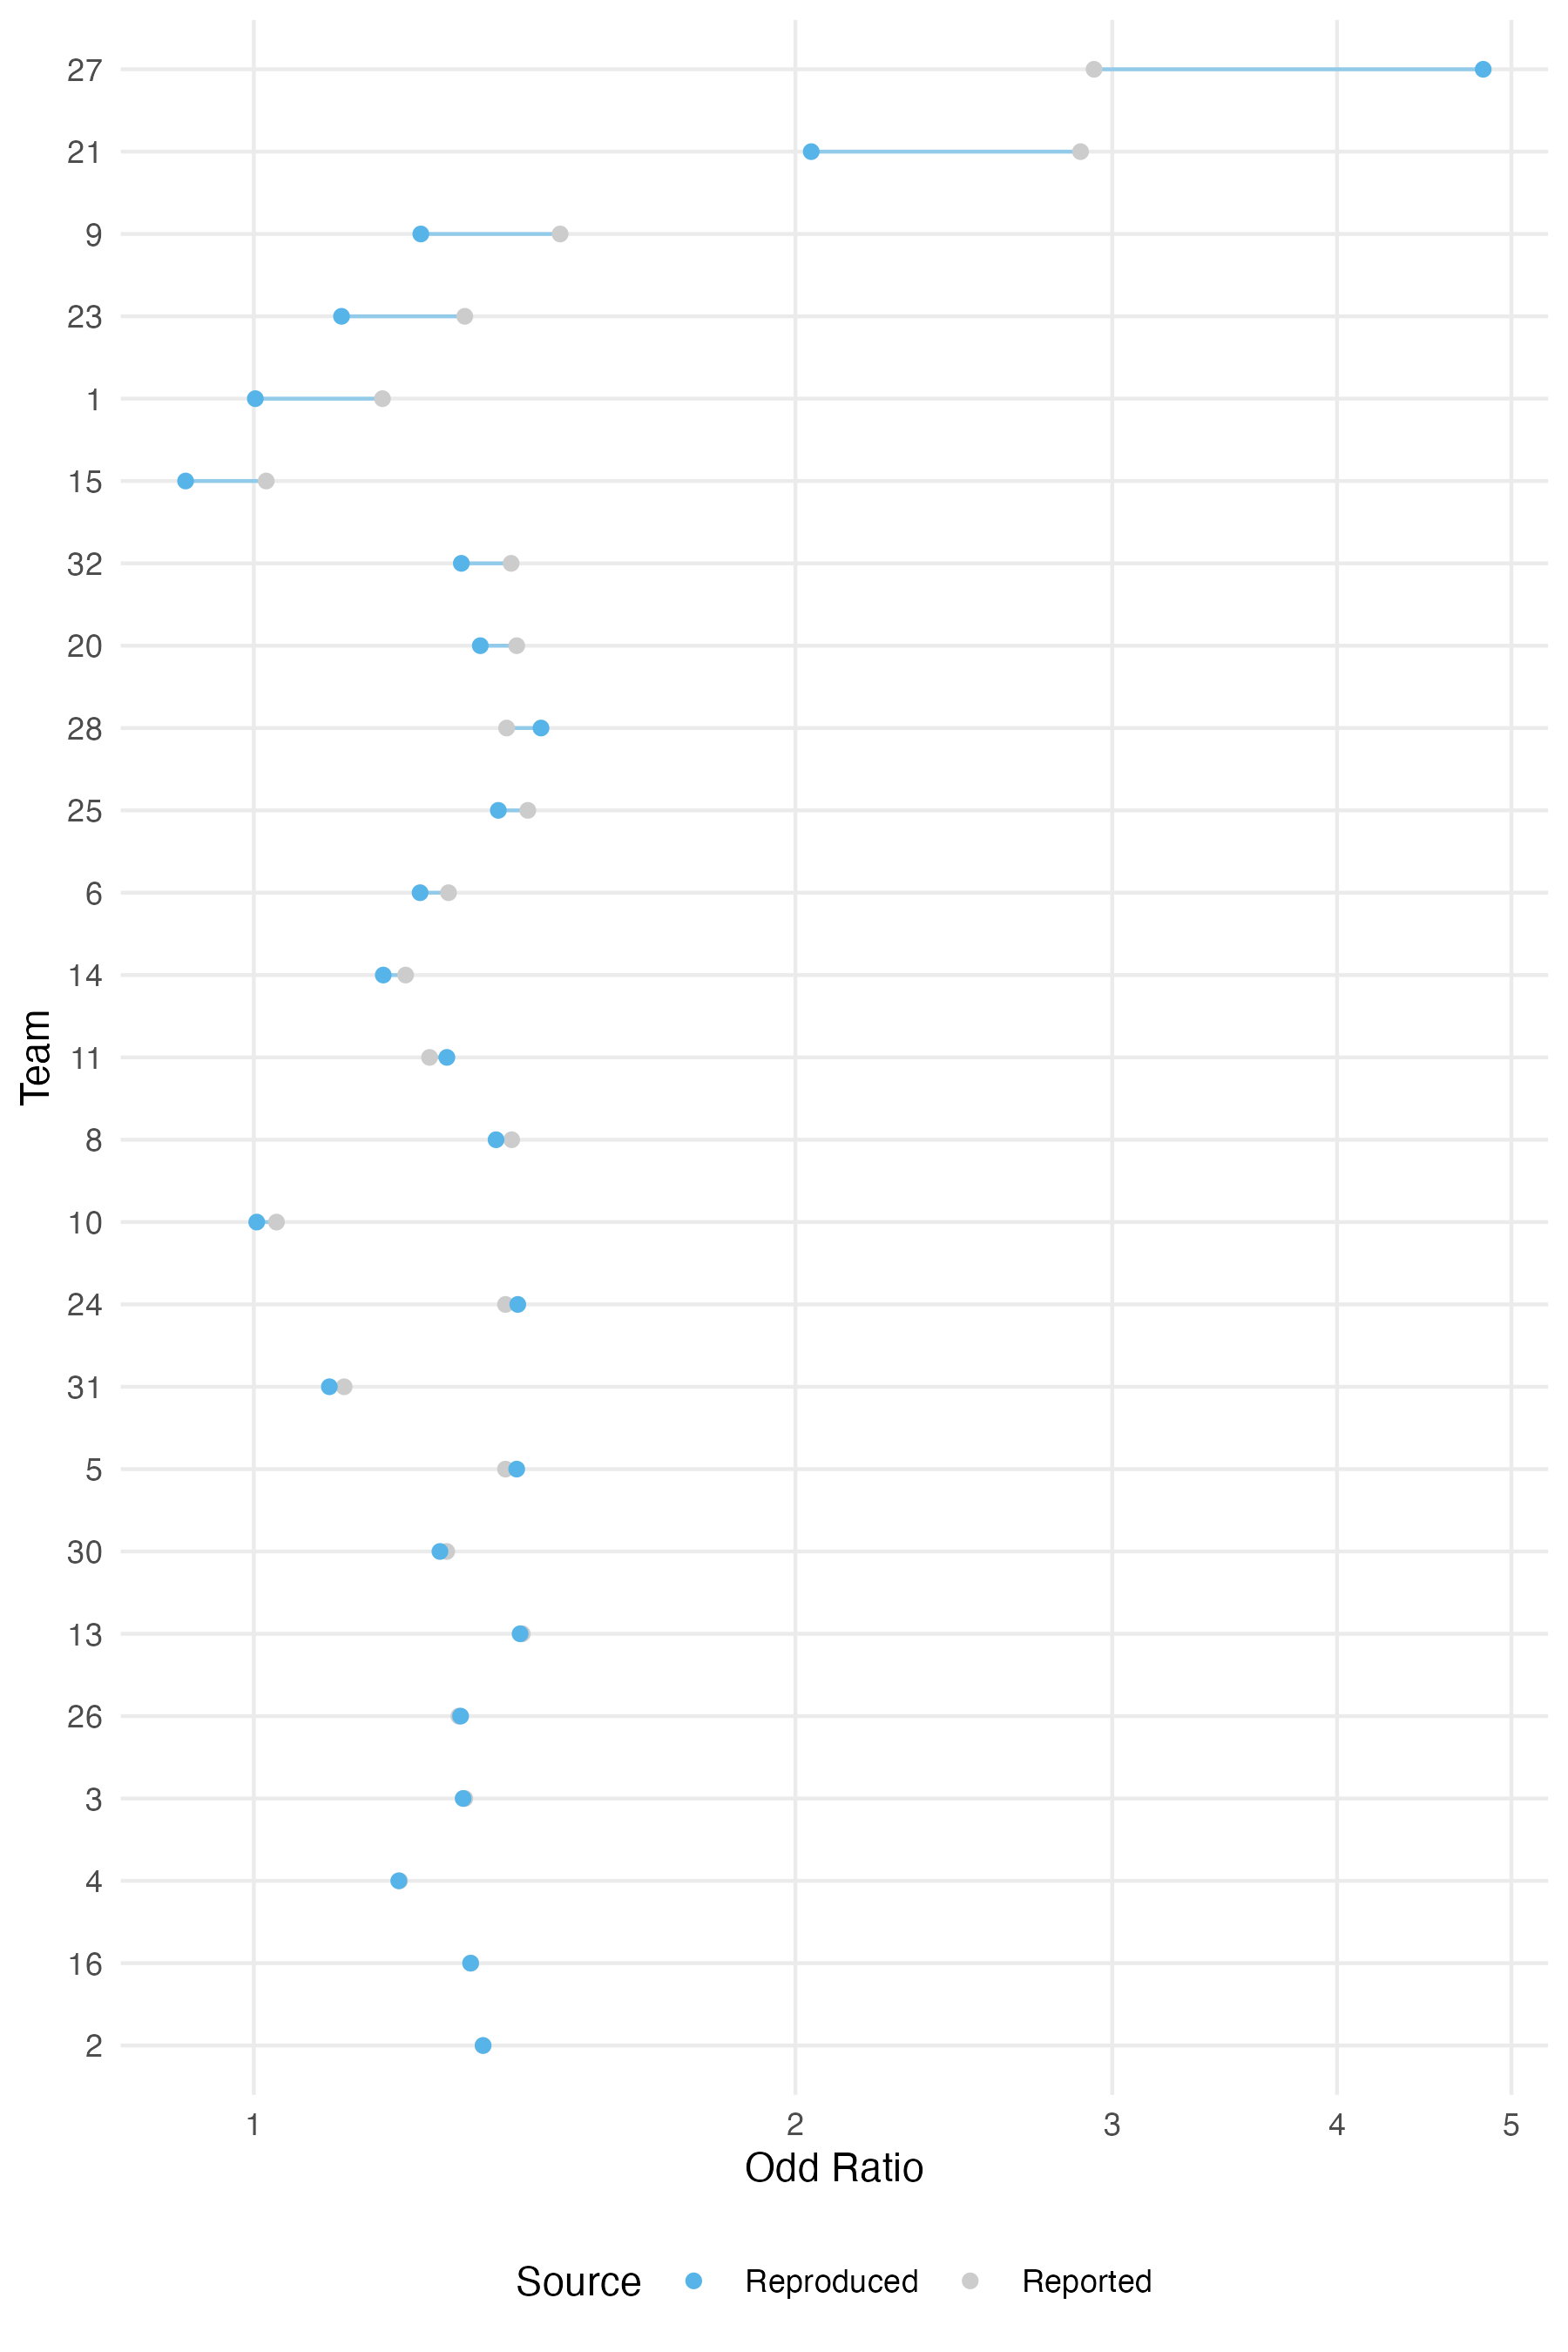
\includegraphics[width=0.9\linewidth,height=0.8\textheight]{figures/res-schema.png}

}

\caption{\label{fig-res-schema}Comparison of the odds ratio of the
effect of skin color on receiving red cards in football games from our
schema-based reproduction (reproduced) vs.~the effect size reported in
Silberzahn et al. (2018) (reported). Teams are ordered by the absolute
difference between the reproduced and reported odds ratio. The
reproduction recovers the reported odds ratio closely for most teams;
the largest deviations occur for Team 1, 9, 15, 21, 23, and 27.}

\end{figure}%

Figure~\ref{fig-res-schema} shows the comparison of the estimated effect
sizes, in odds ratio, from our workflow (reproduced) and those reported
in Silberzahn et al. (2018) (reported). The odds ratio is well recovered
for most teams, though six show a noticeably larger gap: Team 1, 9, 15,
21, 23, and 27. Each of these is worth examining, and the schema is what
makes the examination possible: because the extracted decisions can be
inspected before any code is written, a discrepancy can be attributed to
the report, to the code generated from it, or to neither.

Two of the six are properties of the report rather than of our pipeline.
Team 9 is the clearest: the text names ``referee country'' as the
covariate, while the reported estimation table lists ``player country''.
The report contradicts itself, and no reading of the manuscript can
settle which model produced the published estimate. Team 27 is ambiguous
rather than contradictory. The authors write: ``In addition to the
independent variables specified in the initial approach, \ldots{} a
variable for player position was included, as well as a variable for the
league of the player.'' A statistician might reasonably read this as
shorthand for extending the model with interactions, consistent with how
the other covariates entered the initial model; read literally, it adds
only main effects. The schema records what the text says in both cases,
and the discrepancy that follows is the test's finding, not its failure:
these are the two reports whose description of the analysis is not
sufficient to regenerate the result.

The confidence score \(\omega_i\) separates these two cases in a way
worth noting. For Team 27, extraction returned
\texttt{create\_interaction\_terms} with medium confidence, flagging the
step whose reading is in doubt before any code was written. For Team 9,
every step came back with high confidence, which is the correct response
rather than an oversight: the report's text is unambiguous on its own
terms, and the inconsistency appears only when that text is set against
the estimation table. Since \(\omega_i\) records the model's confidence
that the schema reflects the source text, it can surface a description
that is ambiguous, but not one that is internally clear and contradicted
elsewhere. Catching the latter requires comparing the schema against the
reported results, which is what the test as a whole does.

Teams 1 and 23 are failures of a different kind, and they are ours: the
schema is right and the code is wrong. Both require reshaping the data
from player-referee pairs to individual games, disaggregating
win/loss/draw counts into game-level records. The schema correctly
specifies this step, but the generated code fails to execute it as
intended, and the resulting error passes through validation silently
rather than triggering a repair.

Team 15's discrepancy is unrelated to either stage: it comes down to a
difference in default contrast coding between R (our reproduction) and
SPSS (the original analysis) --- SPSS's effect coding compares each
level to the grand mean, while R's default dummy coding compares to a
reference level. Setting the \texttt{contrast} option in R to match
recovers the reported odds ratio exactly, so this reflects a software
convention rather than a modeling or LLM error.

That leaves Team 21, whose discrepancy we have been unable to explain.
Examining both the extracted schema and the generated code turned up
nothing that accounts for the gap, and we report it as unresolved rather
than assign it to a cause we cannot establish; the procedure localizes
most discrepancies, but evidently not all of them. Setting Team 21
aside, the five remaining discrepancies divide into two whose reports
cannot be resolved to a single analysis, two where our code generation
failed, and one that reflects a difference in software convention. Only
the middle pair are errors in the workflow itself; the first two are
what the test was built to surface.

\subsection{Exploring alternatives}\label{exploring-alternatives}

During the modelling process, researchers may consider a range of
alternative specifications, such as different covariate and random
effects structures, before arriving at a final model. This can be seen
as a set of alternative decisions within the same modelling step, which
fits naturally into the schema workflow described in
Section~\ref{sec-alternative}. As an example, we return to Team 5, whose
analysis was described above. Having settled on a binomial GLMM with a
logit link for the probability that a player receives a red card in a
single game, Team 5 tests three random effect structures:

\begin{align*}
\textbf{Model 1 (gm1):} \quad \text{logit}(p_{ijk}) &= \beta_0 + \beta_1 X_{ijk} + u_{j} + v_{k} \\
u_{j} &\sim N(0, \sigma^2_{\text{player}}), \quad v_{k} \sim N(0, \sigma^2_{\text{ref}}) \\[1.5em]
\textbf{Model 2 (gm2):} \quad \text{logit}(p_{ijk}) &= \beta_0 + \beta_1 X_{ijk} + u_{j} + v_{0k} + v_{1k} X_{ijk} \\
u_{j} &\sim N(0, \sigma^2_{\text{player}}), \quad \mathbf{v}_{k} \sim N\left(\mathbf{0}, \boldsymbol{\Sigma}_{\text{ref}}\right) \\[1.5em]
\textbf{Model 3 (gm3):} \quad \text{logit}(p_{ijkm}) &= \beta_0 + \beta_1 X_{ijkm} + u_{j} + v_{k} + w_{0m} + w_{1m} X_{ijkm} \\
u_{j} &\sim N(0, \sigma^2_{\text{player}}), \quad v_{k} \sim N(0, \sigma^2_{\text{ref}}), \quad \mathbf{w}_{m} \sim N\left(\mathbf{0}, \boldsymbol{\Sigma}_{\text{country}}\right)
\end{align*}

where \(p\) denotes the probability of a player receiving a red card,
and \(X\) represents the player's skin tone rating. The subscripts
\(i, j, k,\) and \(m\) index the individual observation, player,
referee, and the referee's home country, respectively. The parameter
\(\beta_0\) represents the global baseline log-odds of receiving a red
card, and \(\beta_1\) estimates the fixed effect of a player's skin
tone. The random effects include

\begin{itemize}
\tightlist
\item
  a random intercept for players,
  \(u_j \sim N(0, \sigma^2_{\text{player}})\), in Models 1, 2, and 3,
\item
  a random intercept for referees,
  \(v_k \sim N(0, \sigma^2_{\text{ref}})\), in Models 1 and 3, plus an
  additional random slope for referees in Model 2, and
\item
  a random intercept and slope for referee countries,
  \(\mathbf{w}_{m} \sim N\left(\mathbf{0}, \boldsymbol{\Sigma}_{\text{country}}\right)\),
  in Model 3.
\end{itemize}

All three are specified in a single YAML file, following the format
described in Section~\ref{sec-alternative} and shown in
Listing~\ref{lst-yaml-alternative}. Merging it with Team 5's schema
produces one schema per alternative, and each is passed through the same
code generation and validation used for the original, yielding three
validated scripts from one file and no hand-editing of the team's code.
The estimated effect of skin tone is unchanged across this expansion,
matching the value Team 5 report and shown for this team in
Figure~\ref{fig-res-schema}.

\begin{codelisting}

\caption{\label{lst-yaml-alternative}Example of a YAML file specifying
alternatives for the random effects structure in the many-analysts
analysis of Team 5.}

\centering{

\begin{Shaded}
\begin{Highlighting}[]
\FunctionTok{meta}\KeywordTok{:}
\AttributeTok{  }\FunctionTok{type}\KeywordTok{:}\AttributeTok{ alternatives}
\AttributeTok{  }\FunctionTok{branch}\KeywordTok{:}\AttributeTok{ multi}
\FunctionTok{nodes}\KeywordTok{:}
\KeywordTok{{-}}\AttributeTok{ }\FunctionTok{overrides}\KeywordTok{:}\AttributeTok{ specify\_random\_effects\_structure}
\AttributeTok{  }\FunctionTok{alternatives}\KeywordTok{:}
\AttributeTok{  }\KeywordTok{{-}}\AttributeTok{ }\FunctionTok{id}\KeywordTok{:}\AttributeTok{ gm1}
\AttributeTok{    }\FunctionTok{decision}\KeywordTok{:}\AttributeTok{ a random effect of player and referee}
\AttributeTok{    }\FunctionTok{rationale}\KeywordTok{:}\AttributeTok{ }\StringTok{\textquotesingle{}\textquotesingle{}}
\AttributeTok{  }\KeywordTok{{-}}\AttributeTok{ }\FunctionTok{id}\KeywordTok{:}\AttributeTok{ gm2}
\AttributeTok{    }\FunctionTok{decision}\KeywordTok{:}\AttributeTok{ a random effect of player and referee, and a random effect of skin{-}tone across referees}
\AttributeTok{    }\FunctionTok{rationale}\KeywordTok{:}\AttributeTok{ }\StringTok{\textquotesingle{}\textquotesingle{}}
\AttributeTok{  }\KeywordTok{{-}}\AttributeTok{ }\FunctionTok{id}\KeywordTok{:}\AttributeTok{ gm3}
\AttributeTok{    }\FunctionTok{decision}\KeywordTok{:}\AttributeTok{ a random effect of player, referee, and referees\textquotesingle{} countries of origin, and a random effect of skin tone across referees\textquotesingle{} countries of origin}
\AttributeTok{    }\FunctionTok{rationale}\KeywordTok{:}\AttributeTok{ }\StringTok{\textquotesingle{}\textquotesingle{}}
\end{Highlighting}
\end{Shaded}

}

\end{codelisting}%

\section{Discussion}\label{sec-discussion}

Our results highlight a persistent gap between computational
reproducibility and analytical understandability in modern data analysis
workflows. Current reproducibility practices ensure that published
results can be regenerated from shared data and code, but as analyses
grow in complexity and involve iterative decision-making, they fall well
short of making those analyses understandable to readers. Our proposed
schema addresses this gap by introducing an intermediate representation
that explicitly encodes analytical decisions to bridge between narrative
descriptions and implementation details. When coupled with LLMs, this
representation enables the extraction of analytical structure from
written reports, its translation into analysis scripts, and the
exploration of alternative analytical choices.

Our approach differs in this respect from recent work that builds fully
automated systems using multiple LLM agents to plan, generate, execute,
and refine data analyses (Hu et al., 2024; Jansen et al., 2025). These
systems rely on the same underlying capability of translating analytical
specifications into code that our workflow uses, but they aim to
automate the analytical decisions themselves, not just their translation
into code. The failure modes we document in
Section~\ref{sec-application} suggest this is premature: even the
comparatively narrower task of translating an already-specified decision
into working code is not yet fully reliable. We take this as support for
our position that the harder and more consequential part of a data
analysis is the sequence of decisions a researcher makes, not the code
that implements them, and that this part should remain explicit and in
the hands of the analyst rather than be automated away.

Where no schema is supplied, the same workflow serves as a
reproducibility test, and we apply it in this form to the many-analysts
football study. It surfaces inconsistencies and ambiguities in the
original reports that computational reproducibility alone would not
catch: Team 9's report names one covariate in its text and a different
one in its estimation table, a contradiction that is invisible if one
only re-runs the authors' code, and that only becomes apparent once the
described analysis is written down as an explicit set of decisions and
executed. Examining the largest discrepancies also separates defects in
the reports from failures of our own pipeline --- two of each, with a
fifth attributable to a difference in software convention. The
separation is possible because the schema sits between the manuscript
and the code and can be checked against the manuscript on its own, and
it matters for where effort should be directed: an unresolvable report
calls for disambiguation at the source, and the confidence score
\(\omega_i\) is the natural hook for it, having flagged the disputed
step in Team 27's report before any code was written, whereas a
code-generation failure calls for improvements to the validation stage
itself.

A caveat applies to the failure modes we report: they describe the
behaviour of one model at one point in time. Current models parse
methodology text reliably for the most part, and where they slip is on
statistical nuance that a trained reader supplies without thinking. The
phrase ``a random effect of referee number across average rating'' would
be read by most statisticians as implying both a random intercept and a
random slope; read literally, as the model reads it, it specifies a
random slope only. This points to a gap between current models and human
analysts in specialized statistical knowledge (Sun et al., 2026), but
given the pace at which these models are improving we expect this
particular gap to narrow, and we do not regard it as a structural
limitation of the workflow. What the workflow provides, independently of
model capability, is somewhere to catch such a misreading: the schema is
inspectable before any code is generated, so a misread decision is
visible to the analyst as a sentence rather than buried in a script.

Our validate-and-repair loop assumes each candidate script can be
executed and diagnosed within an interactive timeframe. This assumption
does not hold for analyses that are too computationally expensive to run
inside such a loop (Teams 7, 12, 17, and 18 in the many-analysts
football study). As a future direction, this could be addressed by
implementing a background job queue to allow longer-running scripts to
be executed asynchronously.

Turning to the other stage, the validation loop successfully corrects a
range of implementation issues, including errors caused by overflowing
comments and other syntax problems. What it does not catch are
transformations that run without error but do not do what the schema
asked, of which the reshaping failures behind Teams 1 and 23 are the
clearest instance: changing the unit of analysis from player-referee
dyads to individual games produces code that executes and returns an
estimate regardless of whether the disaggregation was done correctly. We
also observe some difficulties in parsing birthdates. Since the LLM does
not have access to the underlying raw data, due to privacy constraints,
it must rely on trial and error when inferring the correct date format,
in this case ``DD-MM-YYYY''. This suggests that certain types of data
analysis tasks may not be fully automatable in settings where the model
cannot directly inspect the data, even if the data is theoretically
available for computation.

While the schema requires a rationale \(\rho_i\) for each decision,
nothing in the format itself can guarantee that this rationale is
substantive rather than perfunctory; an analyst can satisfy the schema
with a low-effort entry in the same way that a required code comment or
commit message can be filled with boilerplate. The schema makes
recording a decision's rationale cheap and structured, but, as with any
documentation requirement, cannot enforce that authors use it
thoughtfully. It remains an open question whether resolving
\(\mathcal{I}_i\) and \(\mathcal{O}_i\) to concrete dataset variables
ahead of time, rather than leaving this mapping for the LLM to infer at
the point of code generation, meaningfully improves the reliability of
the resulting code.

The reproducibility-understandability issue considered in this work is
still at an early stage, and some software design choices are worth
examining. We currently implement a prototype as an R package, although
the understandability problem is broadly applicable to statistical
analyses and is not associated with any particular programming language.
Hence, we envision the implementation eventually evolving into a general
purpose tool, such as a command-line utility, that can support analyses
across different programming languages. In the current implementation,
analytical decisions are recorded in a single YAML file. An alternative
would be to record individual decisions in separate Markdown files.
While YAML files provide an explicit structure for machine readability,
Markdown files offer greater flexibility for documenting decisions.
Recording decisions in separate files would also allow them to be linked
across time, showing how decisions evolve over the course of an
analysis. This could in turn support a broader research-management
system, provided that decisions are properly attributed to individual
researchers and that a record of the changes leading to the final
analysis is maintained.

\section{Acknowledgments}\label{acknowledgments}

The implementation of the schema is available on CRAN as an R package,
\texttt{tines}. The source code for reproducing the work reported in
this paper is available in the Supplementary Materials and can be found
at: \url{https://github.com/huizezhang-sherry/paper-schema}.

All analyses were carried out in R (R Core Team, 2026), using the
\texttt{tines}, \texttt{tidyverse} (Wickham et al., 2019), \texttt{VGAM}
(Yee, 2025), \texttt{VGAMdata} (Yee \& Gray, 2025), \texttt{lme4} (Bates
et al., 2015), \texttt{glmmTMB} (Brooks et al., 2017; McGillycuddy et
al., 2025), and \texttt{fixest} (Bergé et al., 2026) packages. The
article is created using Quarto (Allaire et al., 2026).

\section*{References}\label{references}
\addcontentsline{toc}{section}{References}

\phantomsection\label{refs}
\begin{CSLReferences}{1}{0}
\bibitem[\citeproctext]{ref-Allaire_Quarto_2026}
Allaire, J. J., Teague, C., Scheidegger, C., Xie, Y., Dervieux, C., \&
Woodhull, G. (2026). \emph{{Quarto}} (Version 1.9) {[}Computer
software{]}. \url{https://doi.org/10.5281/zenodo.5960048}

\bibitem[\citeproctext]{ref-lme4}
Bates, D., Mächler, M., Bolker, B., \& Walker, S. (2015). Fitting linear
mixed-effects models using {lme4}. \emph{Journal of Statistical
Software}, \emph{67}(1), 1--48.
\url{https://doi.org/10.18637/jss.v067.i01}

\bibitem[\citeproctext]{ref-fixest}
Bergé, L. R., Butts, K., \& McDermott, G. (2026). Fast and user-friendly
econometrics estimations: {T}he {R} package fixest. \emph{arXiv Preprint
arXiv:2601.21749}. \url{https://doi.org/10.48550/arXiv.2601.21749}

\bibitem[\citeproctext]{ref-glmmTMB-1}
Brooks, M. E., Kristensen, K., van Benthem, K. J., Magnusson, A., Berg,
C. W., Nielsen, A., Skaug, H. J., Maechler, M., \& Bolker, B. M. (2017).
{glmmTMB} balances speed and flexibility among packages for
zero-inflated generalized linear mixed modeling. \emph{The R Journal},
\emph{9}(2), 378--400. \url{https://doi.org/10.32614/RJ-2017-066}

\bibitem[\citeproctext]{ref-hu_automated_2024}
Hu, S., Lu, C., \& Clune, J. (2024, October). \emph{Automated {Design}
of {Agentic} {Systems}}.
\url{https://openreview.net/forum?id=t9U3LW7JVX}

\bibitem[\citeproctext]{ref-jansen2025}
Jansen, J. A., Manukyan, A., Khoury, N. A., \& Akalin, A. (2025).
Leveraging large language models for data analysis automation.
\emph{PLOS ONE}, \emph{20}(2), e0317084.
\url{https://doi.org/10.1371/journal.pone.0317084}

\bibitem[\citeproctext]{ref-glmmTMB-2}
McGillycuddy, M., Warton, D. I., Popovic, G., \& Bolker, B. M. (2025).
Parsimoniously fitting large multivariate random effects in {glmmTMB}.
\emph{Journal of Statistical Software}, \emph{112}(1), 1--19.
\url{https://doi.org/10.18637/jss.v112.i01}

\bibitem[\citeproctext]{ref-peng_reproducible_2011}
Peng, R. D. (2011). Reproducible {Research} in {Computational}
{Science}. \emph{Science}, \emph{334}(6060), 1226--1227.
\url{https://doi.org/10.1126/science.1213847}

\bibitem[\citeproctext]{ref-R}
R Core Team. (2026). \emph{R: A language and environment for statistical
computing}. R Foundation for Statistical Computing.
\url{https://doi.org/10.32614/R.manuals}

\bibitem[\citeproctext]{ref-sarma2023}
Sarma, A., Kale, A., Moon, M. J., Taback, N., Chevalier, F., Hullman,
J., \& Kay, M. (2023). Multiverse: Multiplexing alternative data
analyses in r notebooks. \emph{Proceedings of the 2023 CHI Conference on
Human Factors in Computing Systems}.
\url{https://doi.org/10.1145/3544548.3580726}

\bibitem[\citeproctext]{ref-silberzahn2018}
Silberzahn, R., Uhlmann, E. L., Martin, D. P., Anselmi, P., Aust, F.,
Awtrey, E., Bahník, Š., Bai, F., Bannard, C., Bonnier, E., Carlsson, R.,
Cheung, F., Christensen, G., Clay, R., Craig, M. A., Dalla Rosa, A.,
Dam, L., Evans, M. H., Flores Cervantes, I., \ldots{} Nosek, B. A.
(2018). Many Analysts, One Data Set: Making Transparent How Variations
in Analytic Choices Affect Results. \emph{Advances in Methods and
Practices in Psychological Science}, \emph{1}(3), 337--356.
\url{https://doi.org/10.1177/2515245917747646}

\bibitem[\citeproctext]{ref-sun_lambda_2026}
Sun, M., Han, R., Jiang, B., Qi, H., Sun, D., Yuan, Y., \& Huang, J.
(2026). {LAMBDA}: {A} {Large} {Model} {Based} {Data} {Agent}.
\emph{Journal of the American Statistical Association}, \emph{121},
1--13. \url{https://doi.org/10.1080/01621459.2025.2510000}

\bibitem[\citeproctext]{ref-hdi}
United Nations Development Programme. (2025). \emph{Human development
report 2025}. United Nations Development Programme.
\url{https://hdr.undp.org/}

\bibitem[\citeproctext]{ref-wickham2019tidyverse}
Wickham, H., Averick, M., Bryan, J., Chang, W., McGowan, L. D.,
François, R., Grolemund, G., Hayes, A., Henry, L., Hester, J., Kuhn, M.,
Pedersen, T. L., Miller, E., Bache, S. M., Müller, K., Ooms, J.,
Robinson, D., Seidel, D. P., Spinu, V., \ldots{} Yutani, H. (2019).
Welcome to the tidyverse. \emph{Journal of Open Source Software},
\emph{4}(43), 1686. \url{https://doi.org/10.21105/joss.01686}

\bibitem[\citeproctext]{ref-wrobel_partnering_2024}
Wrobel, J., Hector, E. C., Crawford, L., McGowan, L. D., Silva, N. da,
Goldsmith, J., Hicks, S., Kane, M., Lee, Y., Mayrink, V., Paciorek, C.
J., Usher, T., \& Wolfson, J. (2024). Partnering {With} {Authors} to
{Enhance} {Reproducibility} at {JASA}. \emph{Journal of the American
Statistical Association}, \emph{119}(546), 795--797.
\url{https://doi.org/10.1080/01621459.2024.2340557}

\bibitem[\citeproctext]{ref-VGAM}
Yee, T. W. (2025). \emph{{VGAM}: Vector generalized linear and additive
models}. \url{https://CRAN.R-project.org/package=VGAM}

\bibitem[\citeproctext]{ref-yee2025heaping}
Yee, T. W., Frigau, L., \& Ma, C. (2025). Heaping and seeping, GAITD
regression and doubly constrained reduced-rank vector generalized linear
models in smoking studies. \emph{The Annals of Applied Statistics},
\emph{19}(4), 3045--3070.

\bibitem[\citeproctext]{ref-VGAMdata}
Yee, T. W., \& Gray, J. (2025). \emph{{VGAMdata}: Data supporting the
{VGAM} package}. \url{https://CRAN.R-project.org/package=VGAMdata}

\end{CSLReferences}




\end{document}
